% Options for packages loaded elsewhere
\PassOptionsToPackage{unicode}{hyperref}
\PassOptionsToPackage{hyphens}{url}
%
\documentclass[
  english,
  doc,floatsintext]{apa6}
\usepackage{amsmath,amssymb}
\usepackage{lmodern}
\usepackage{iftex}
\ifPDFTeX
  \usepackage[T1]{fontenc}
  \usepackage[utf8]{inputenc}
  \usepackage{textcomp} % provide euro and other symbols
\else % if luatex or xetex
  \usepackage{unicode-math}
  \defaultfontfeatures{Scale=MatchLowercase}
  \defaultfontfeatures[\rmfamily]{Ligatures=TeX,Scale=1}
\fi
% Use upquote if available, for straight quotes in verbatim environments
\IfFileExists{upquote.sty}{\usepackage{upquote}}{}
\IfFileExists{microtype.sty}{% use microtype if available
  \usepackage[]{microtype}
  \UseMicrotypeSet[protrusion]{basicmath} % disable protrusion for tt fonts
}{}
\makeatletter
\@ifundefined{KOMAClassName}{% if non-KOMA class
  \IfFileExists{parskip.sty}{%
    \usepackage{parskip}
  }{% else
    \setlength{\parindent}{0pt}
    \setlength{\parskip}{6pt plus 2pt minus 1pt}}
}{% if KOMA class
  \KOMAoptions{parskip=half}}
\makeatother
\usepackage{xcolor}
\IfFileExists{xurl.sty}{\usepackage{xurl}}{} % add URL line breaks if available
\IfFileExists{bookmark.sty}{\usepackage{bookmark}}{\usepackage{hyperref}}
\hypersetup{
  pdftitle={No evidence that age affects different bilingual learner groups differently: Rebuttal to van der Slik, Schepens, Bongaerts, and van Hout (2021)},
  pdfauthor={Joshua K Hartshorne1},
  pdflang={en-EN},
  hidelinks,
  pdfcreator={LaTeX via pandoc}}
\urlstyle{same} % disable monospaced font for URLs
\usepackage{graphicx}
\makeatletter
\def\maxwidth{\ifdim\Gin@nat@width>\linewidth\linewidth\else\Gin@nat@width\fi}
\def\maxheight{\ifdim\Gin@nat@height>\textheight\textheight\else\Gin@nat@height\fi}
\makeatother
% Scale images if necessary, so that they will not overflow the page
% margins by default, and it is still possible to overwrite the defaults
% using explicit options in \includegraphics[width, height, ...]{}
\setkeys{Gin}{width=\maxwidth,height=\maxheight,keepaspectratio}
% Set default figure placement to htbp
\makeatletter
\def\fps@figure{htbp}
\makeatother
\setlength{\emergencystretch}{3em} % prevent overfull lines
\providecommand{\tightlist}{%
  \setlength{\itemsep}{0pt}\setlength{\parskip}{0pt}}
\setcounter{secnumdepth}{-\maxdimen} % remove section numbering
% Make \paragraph and \subparagraph free-standing
\ifx\paragraph\undefined\else
  \let\oldparagraph\paragraph
  \renewcommand{\paragraph}[1]{\oldparagraph{#1}\mbox{}}
\fi
\ifx\subparagraph\undefined\else
  \let\oldsubparagraph\subparagraph
  \renewcommand{\subparagraph}[1]{\oldsubparagraph{#1}\mbox{}}
\fi
\newlength{\cslhangindent}
\setlength{\cslhangindent}{1.5em}
\newlength{\csllabelwidth}
\setlength{\csllabelwidth}{3em}
\newlength{\cslentryspacingunit} % times entry-spacing
\setlength{\cslentryspacingunit}{\parskip}
\newenvironment{CSLReferences}[2] % #1 hanging-ident, #2 entry spacing
 {% don't indent paragraphs
  \setlength{\parindent}{0pt}
  % turn on hanging indent if param 1 is 1
  \ifodd #1
  \let\oldpar\par
  \def\par{\hangindent=\cslhangindent\oldpar}
  \fi
  % set entry spacing
  \setlength{\parskip}{#2\cslentryspacingunit}
 }%
 {}
\usepackage{calc}
\newcommand{\CSLBlock}[1]{#1\hfill\break}
\newcommand{\CSLLeftMargin}[1]{\parbox[t]{\csllabelwidth}{#1}}
\newcommand{\CSLRightInline}[1]{\parbox[t]{\linewidth - \csllabelwidth}{#1}\break}
\newcommand{\CSLIndent}[1]{\hspace{\cslhangindent}#1}
% Manuscript styling
\usepackage{upgreek}
\captionsetup{font=singlespacing,justification=justified}

% Table formatting
\usepackage{longtable}
\usepackage{lscape}
% \usepackage[counterclockwise]{rotating}   % Landscape page setup for large tables
\usepackage{multirow}		% Table styling
\usepackage{tabularx}		% Control Column width
\usepackage[flushleft]{threeparttable}	% Allows for three part tables with a specified notes section
\usepackage{threeparttablex}            % Lets threeparttable work with longtable

% Create new environments so endfloat can handle them
% \newenvironment{ltable}
%   {\begin{landscape}\begin{center}\begin{threeparttable}}
%   {\end{threeparttable}\end{center}\end{landscape}}
\newenvironment{lltable}{\begin{landscape}\begin{center}\begin{ThreePartTable}}{\end{ThreePartTable}\end{center}\end{landscape}}

% Enables adjusting longtable caption width to table width
% Solution found at http://golatex.de/longtable-mit-caption-so-breit-wie-die-tabelle-t15767.html
\makeatletter
\newcommand\LastLTentrywidth{1em}
\newlength\longtablewidth
\setlength{\longtablewidth}{1in}
\newcommand{\getlongtablewidth}{\begingroup \ifcsname LT@\roman{LT@tables}\endcsname \global\longtablewidth=0pt \renewcommand{\LT@entry}[2]{\global\advance\longtablewidth by ##2\relax\gdef\LastLTentrywidth{##2}}\@nameuse{LT@\roman{LT@tables}} \fi \endgroup}

% \setlength{\parindent}{0.5in}
% \setlength{\parskip}{0pt plus 0pt minus 0pt}

% \usepackage{etoolbox}
\makeatletter
\patchcmd{\HyOrg@maketitle}
  {\section{\normalfont\normalsize\abstractname}}
  {\section*{\normalfont\normalsize\abstractname}}
  {}{\typeout{Failed to patch abstract.}}
\patchcmd{\HyOrg@maketitle}
  {\section{\protect\normalfont{\@title}}}
  {\section*{\protect\normalfont{\@title}}}
  {}{\typeout{Failed to patch title.}}
\makeatother
\shorttitle{Rebuttle to van der Slik et al}
\usepackage{lineno}

\linenumbers
\usepackage{csquotes}
\usepackage{wrapfig}
\usepackage{lipsum}
\ifXeTeX
  % Load polyglossia as late as possible: uses bidi with RTL langages (e.g. Hebrew, Arabic)
  \usepackage{polyglossia}
  \setmainlanguage[]{english}
\else
  \usepackage[main=english]{babel}
% get rid of language-specific shorthands (see #6817):
\let\LanguageShortHands\languageshorthands
\def\languageshorthands#1{}
\fi
\ifLuaTeX
  \usepackage{selnolig}  % disable illegal ligatures
\fi

\title{No evidence that age affects different bilingual learner groups differently: Rebuttal to van der Slik, Schepens, Bongaerts, and van Hout (2021)}
\author{Joshua K Hartshorne\textsuperscript{1}}
\date{}


\authornote{

Data and analysis code can be found at {[}URL to be entered prior to publication{]}.

Correspondence concerning this article should be addressed to Joshua K Hartshorne, 522 McGuinn Hall, Boston College, USA. E-mail: \href{mailto:joshua.hartshorne@bc.edu}{\nolinkurl{joshua.hartshorne@bc.edu}}

}

\affiliation{\vspace{0.5cm}\textsuperscript{1} Department of Psychology and Neuroscience, Boston College}

\abstract{
Hartshorne, Tenenbaum, and Pinker (2018, A critical period for second language acquisition: Evidence from 2/3 million English speakers. \emph{Cognition}, 117, 263-277) presented the first direct estimate of how the ability to learn the syntax of a second language changes with age. They accomplished this by applying a novel analytic model to a massive dataset of native and non-native speakers, finding a sharp decline at around 17 years old. Recently, van der Slik, Schepens, Bongaerts, and van Hout (2021, Critical period claim revisited: Reanalysis of Hartshorne, Tenenbaum, and Pinker (2018) suggests steady decline and learner-type differences. \emph{Language} \emph{Learning}) found that Hartshorne et al's (2018) model provided different results when applied to subsets of the data (e.g., only monolinguals), which they take to be a refutation of the original results. While the questions raised by van der Slik et al (2021) are interesting and important, their analytic methods are based on conceptual errors and mathematical mistakes. After correcting these mistakes, their proposed analyses strongly confirm the original conclusions of Hartshorne and colleagues.
}



\begin{document}
\maketitle

\hypertarget{introduction}{%
\section{Introduction}\label{introduction}}

One hardly needs to conduct an experiment to show that people who begin learning language as an adult rarely if ever reach the same level of proficiency as those who start in early childhood, though plenty of experimental data do exist (Birdsong, 2018; Flege, 2019; Hartshorne, 2020). What remains highly controversial is \emph{why}: is poor achievement by later learners due to differences in neural plasticity, motivation, interference from a first language, or something else? These questions have been difficult to resolve because of conflicting results across studies, at least in part because only a handful of studies have the statistical power to produce clear results (Hartshorne, 2020; Vanhove, 2013).

In Hartshorne, Tenenbaum, and Pinker (2018) (henceforth HTP), my colleagues and I reported an additional problem: the method typically used to measure critical periods is unable to do so. Specifically, beginning in the 1970s, most studies have used a retrospective ``ultimate attainment'' method, comparing the linguistic abilities of adults as a function of the age at which they started learning the language in question. Unfortunately, this method turns out to be subject to a number of confounds. Most importantly, very different age-related changes in the ability to learn language can give rise to indistinguishable ultimate attainment curves (Fig. \ref{fig:FigUA}).



\begin{wrapfigure}{R}{0.5\textwidth}
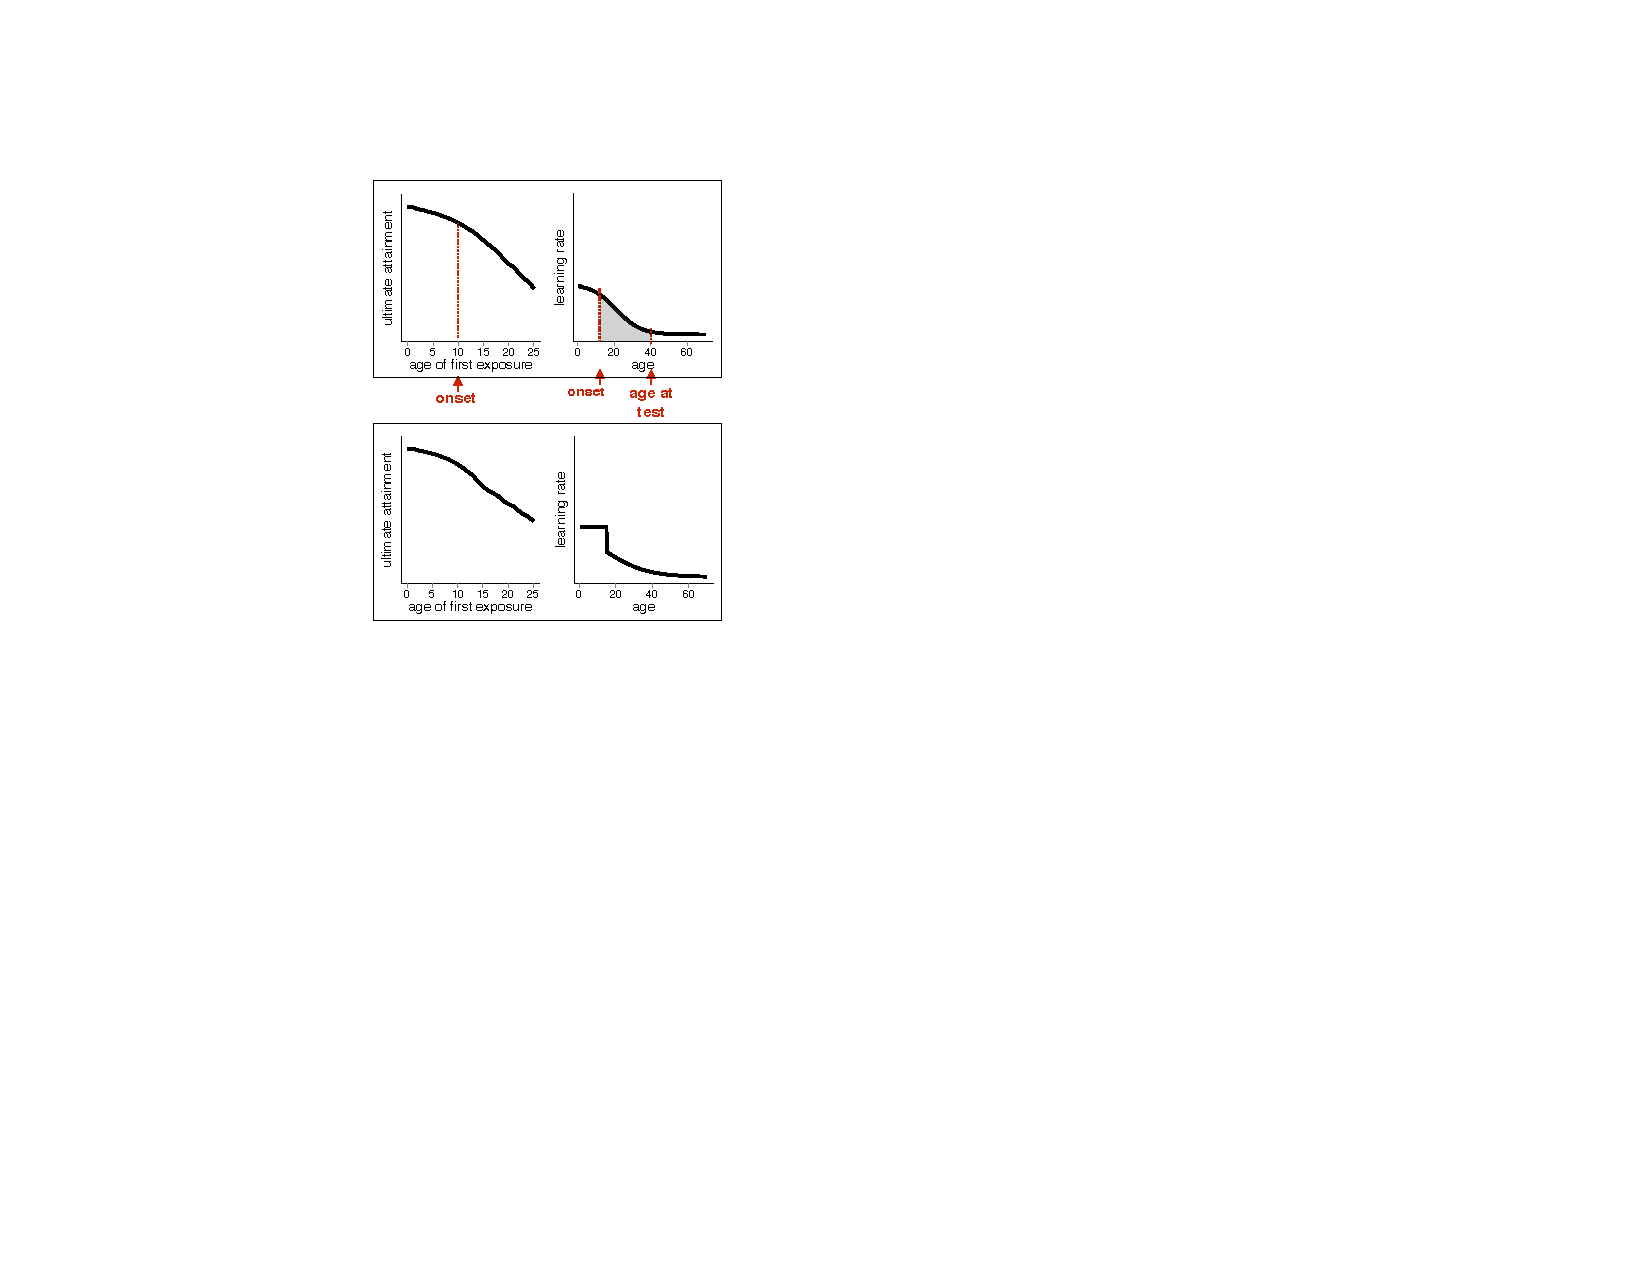
\includegraphics[width=1.5\linewidth]{Figures/FigUA} \caption{Each point on an ultimate attainment curve (\textbf{left panels}) is related to an integral under the learning rate curve (\textbf{right panels}). While most studies have assumed that it is possible to infer the shape of the theoretically-critical learning rate curves from easier-to-measure ultimate attainment curves, these simulations from HTP show that difficult-to-distinguish ultimate attainment curves can actually be explained by very different learning rate curves (\textbf{top} vs.~\textbf{bottom}).}\label{fig:FigUA}
\end{wrapfigure}

The problem is intuitive. Suppose we know that if Agnes leaves her home at 8:15 in the morning, she makes it to work comfortably before 9:00. If she leaves after 8:15, she runs into a traffic jam and arrives much later. Does this mean that the traffic picks up at exactly 8:15? Perhaps. Even a slight decrease in speed, applied over the entire travel distance, could be enough to make her tardy. Alternatively, the traffic may grind to a halt at 8:45, so if Agnes hasn't arrived by then, she is out of luck. The point is that if we know what time she left home and how far she got, we know her \emph{average} speed, but not her speed at any given point along the way.

Similarly, if Bartholomew starts learning Swahili as an adult and manages only 80\% the proficiency of a native speaker, this does not mean that he started out learning more slowly than a Swahili-acquiring infant. In fact, during the initial stages of learning, adults actually learn second languages faster than young children (Snow \& Hoefnagel-Höhle, 1978). All we know for sure is that at some point along the way, his learning rate decayed to the point where he ultimately was unable to get to the finish line.

Thus, studies of ultimate attainment are simply unable to constrain many of the empirical and theoretical disputes about critical periods, which tend to revolve around the age at which learning ability declines and how rapidly it declines.

\hypertarget{the-hartshorne-tenenbaum-pinker-2018-study-htp}{%
\subsection{The Hartshorne, Tenenbaum \& Pinker (2018) Study (HTP)}\label{the-hartshorne-tenenbaum-pinker-2018-study-htp}}

To address this gap, HTP did two things. First, they used a viral grammar quiz to obtain estimate of syntactic knowledge for 669,498 English-speakers. Among these were 246,497 monolinguals, 30,347 simultaneous bilinguals, 14,099 later ``immersion learners'' who learned English in an immigration context, and 258,288 later ``non-immersion learners'' who learned English outside of a predominantly English-speaking country. Second, HTP developed a new analytical model to infer from these data how learning ability changes with age. While the details are available in the original paper, here I walk through the intuition in some detail, since it will be critical for understanding what follows.

First, HTP posited that, all else equal, language-learning can be well-described by exponential decay. That is, how much language a learner learns at any given time is a constant proportion of what is left to be learned. To give some illustrative numbers: instead of learning (say) 20\% each year for 5 years, we learn 20\% the first year, 20\% of the remainder in Year 2 {[}(100\% - 20\%) * 20\% = 16\%{]}, 20\% of the remainder of that in Year 3 {[}(100\% - 20\% - (100\% - 20\%)*20\%) * 20\% = 13\%{]}, and so on. This is an asymptotic process and never quite ends, though in this case there is not much progress after about 20 years. Fitting the results of the monolinguals with an exponential curve, we get a good fit (Fig. \ref{fig:exponentials}, left). The estimated learning rate is 0.13: monolinguals learn an estimated 13\% of whatever is left to learn in a given year.



\begin{figure}
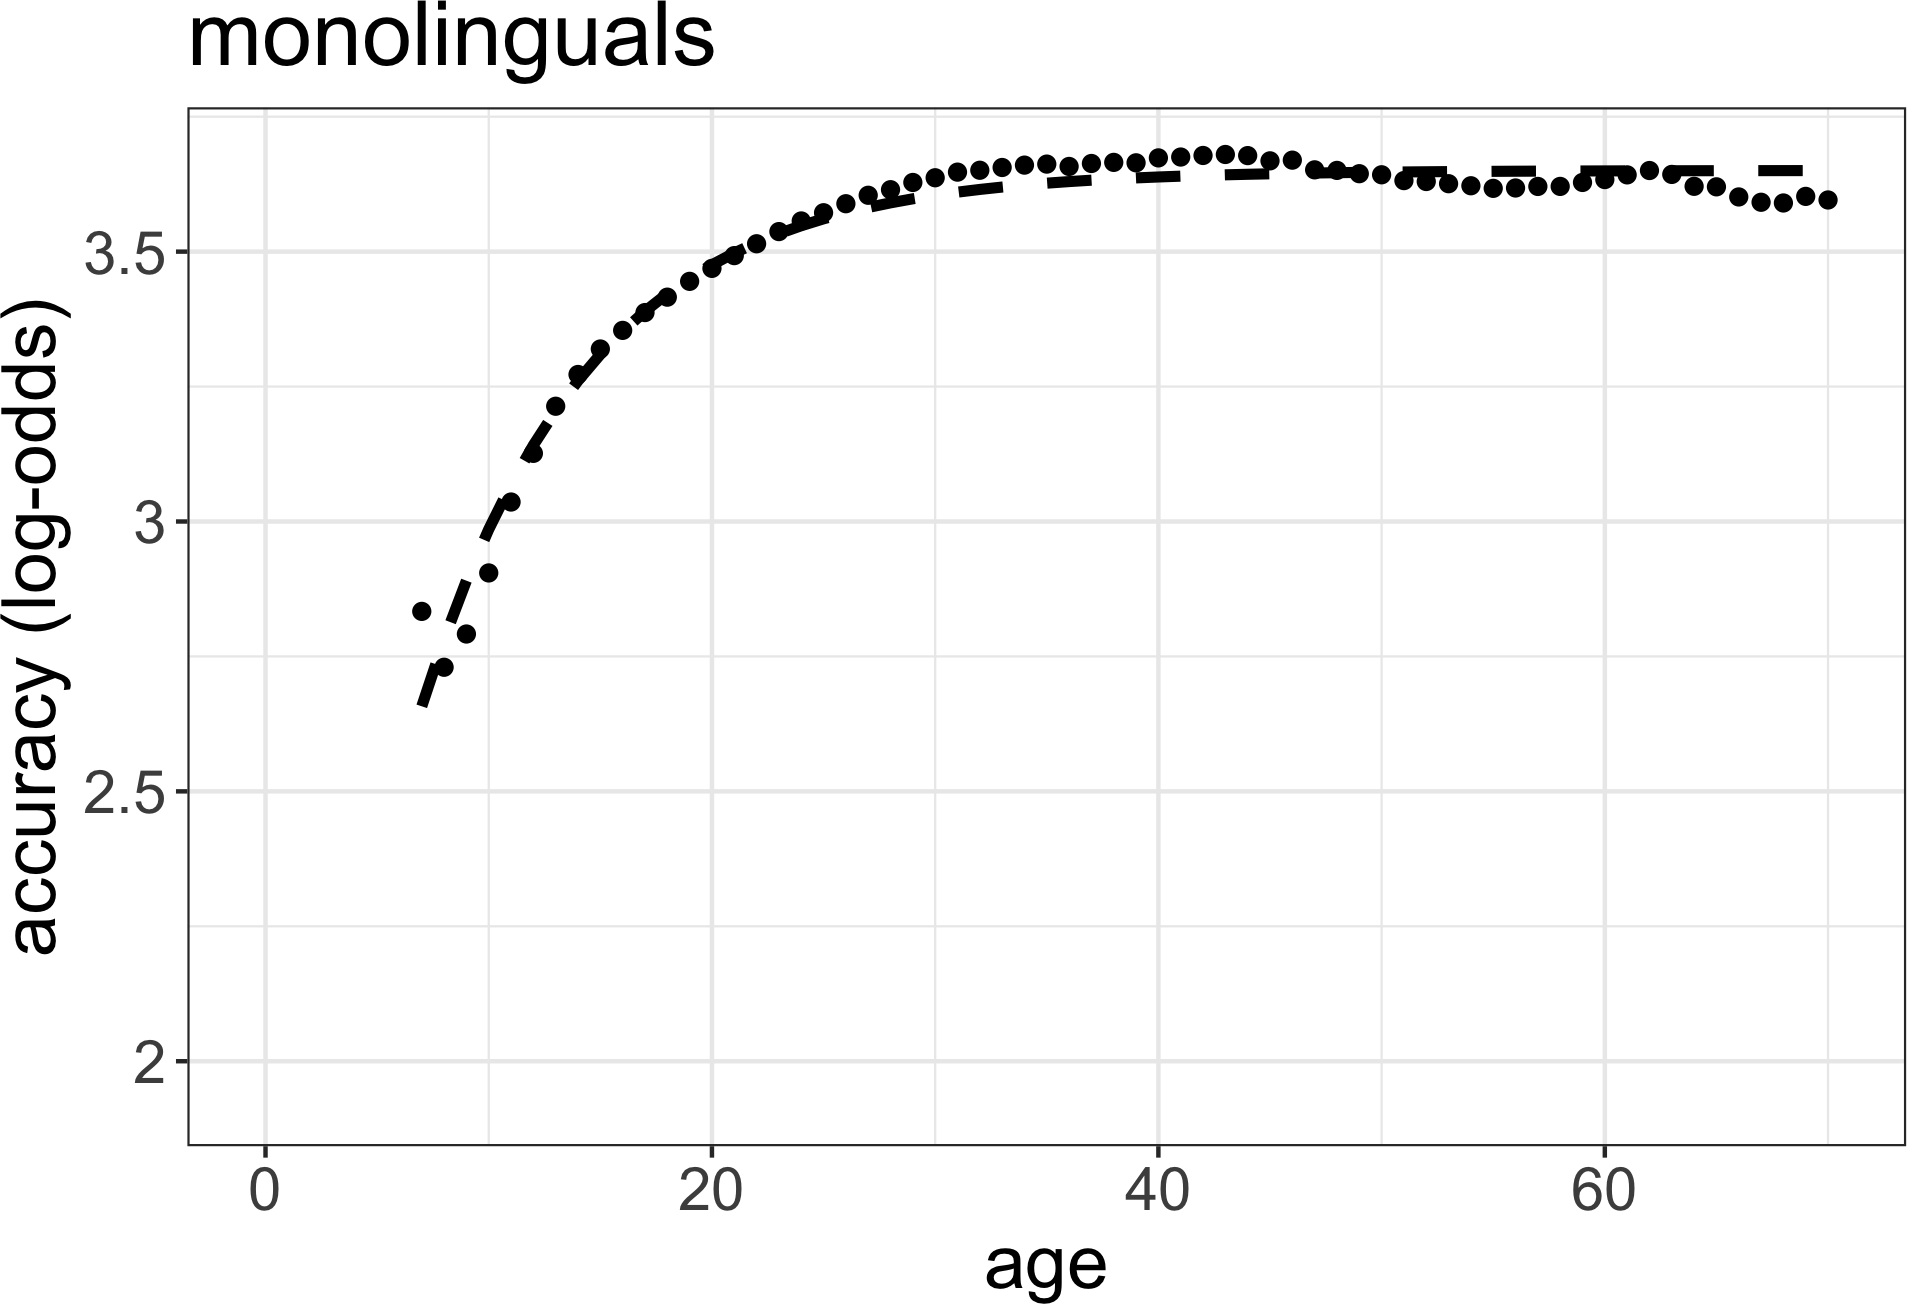
\includegraphics[width=0.45\linewidth]{SlikResponse_rmd_files/figure-latex/exponentials-1} 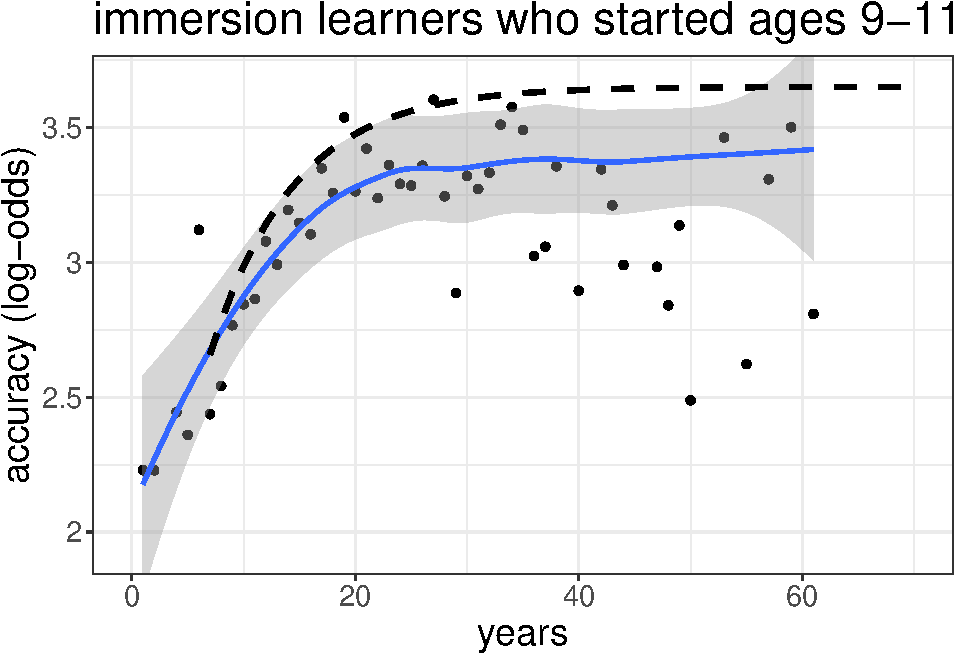
\includegraphics[width=0.45\linewidth]{SlikResponse_rmd_files/figure-latex/exponentials-2} \caption{\textbf{left}: Performance by monolingual English speakers (N=246,497) on HTP's syntax quiz, aggregated by current age. Solid blue line shows the LOESS smooth, with shaded area showing 95\% error bars. Dashed line represents the best-fit exponential decay model. Scale is empirical log-odds (elogit). \textbf{right}: Data from same source, but for learners who began at ages 9-11 and learned in an immersion/immigration setting (N=1373). The dashed line again shows the best-fit exponential decay model \emph{for the monolinguals}. It is clear from the graph that the later learners underperform the monolingual baseline.}\label{fig:exponentials}
\end{figure}

Later learners do not reach the same level as monolingual learners, so their \emph{average} learning rate must be lower. But, as with Agnes's morning commute, that by itself does not tell us where the bottleneck is. As an example, fig.~\ref{fig:exponentials}, right, shows results for learners in HTP's study who began at ages 9-11 and learned in an immersion/immigration setting (N=1373). For comparison, I included the exponential model fit to the monolinguals. Initially, these learners progress perhaps even slightly faster than monolinguals (something that has been observed previously; Snow and Hoefnagel-Höhle (1978)). However, after 15 years, the later learners are noticeably lagging the monolingual pace. Somewhere in between, something changed.

In order to estimate where this change happens, HTP modified the base exponential model to allow the decay (``learning'') rate to change with the learner's biological age. Specifically, they assumed that learning rate is initially flat through some at \(t_c\), after which it declines according to a sigmoid:

\[r(t) = \begin{cases} r_0 & t \leq t_c  \\ r_0(1 - \frac{1}{1+e^{-\alpha*(t - t_e - \delta)}}) & t > t_c
    \end{cases}\]

\noindent where \(r_0\) is the intial learning rate, \(t_e\) is the age of first exposure to English, and \(\alpha\) and \(\delta\) are parameters governing the shape of the sigmoid.

Sigmoids are mathematically convenient (they have few parameters and are integrable, which was critical for this application), but have one substantial drawback: they are symmetric. Thus, if we would like the sigmoid to only gradually approach zero (reflecting the fact that even very old learners can learn at least a little bit), it must begin declining equally gradually (e.g., Fig. \ref{fig:sigmoids}, far left). If we want the onset of the decline to be rapid, then it must approach zero rapidly (e.g., Fig. \ref{fig:sigmoids}, second from left). By having the curve start as a horizontal line, we are able to have sharp initial declines that nonetheless approach zero slowly (e.g., Fig. \ref{fig:sigmoids}, second from right). This has the added advantage of providing a clear demarcation of the critical period (the value of \(t_c\)). (Chen and Hartshorne (2021) present a more elegant formulation that allows for a wider range of asymmetries without the need for a sharp discontinuity in the curve, which we return to below.) HTP's learning curve function also allows for other theoretically-important possibilities, such as no change in learning rate (e.g., Fig. \ref{fig:sigmoids}, far right).



\begin{figure}
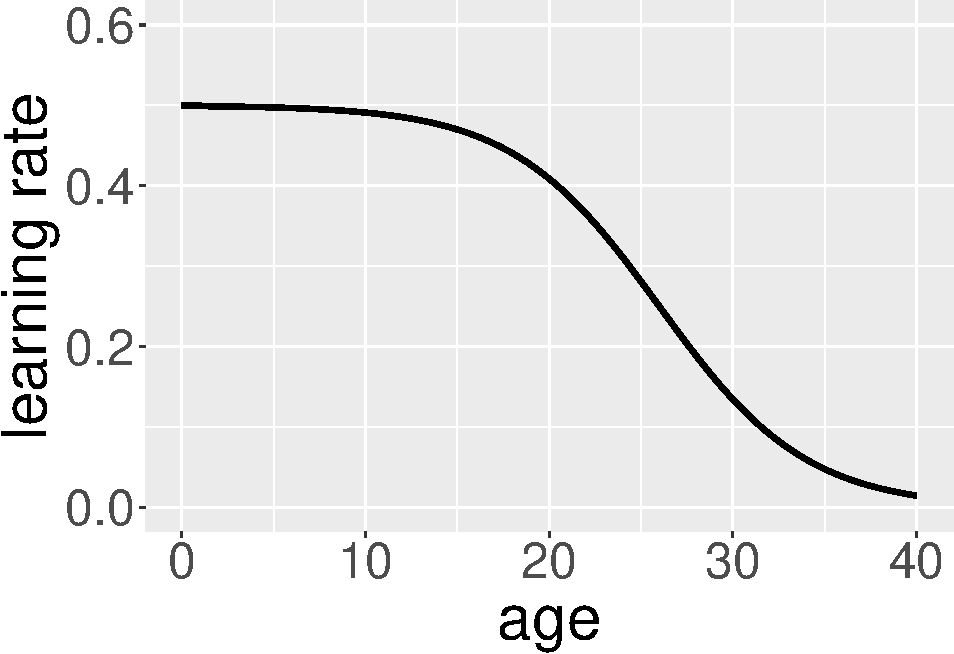
\includegraphics[width=0.24\linewidth]{SlikResponse_rmd_files/figure-latex/sigmoids-1} 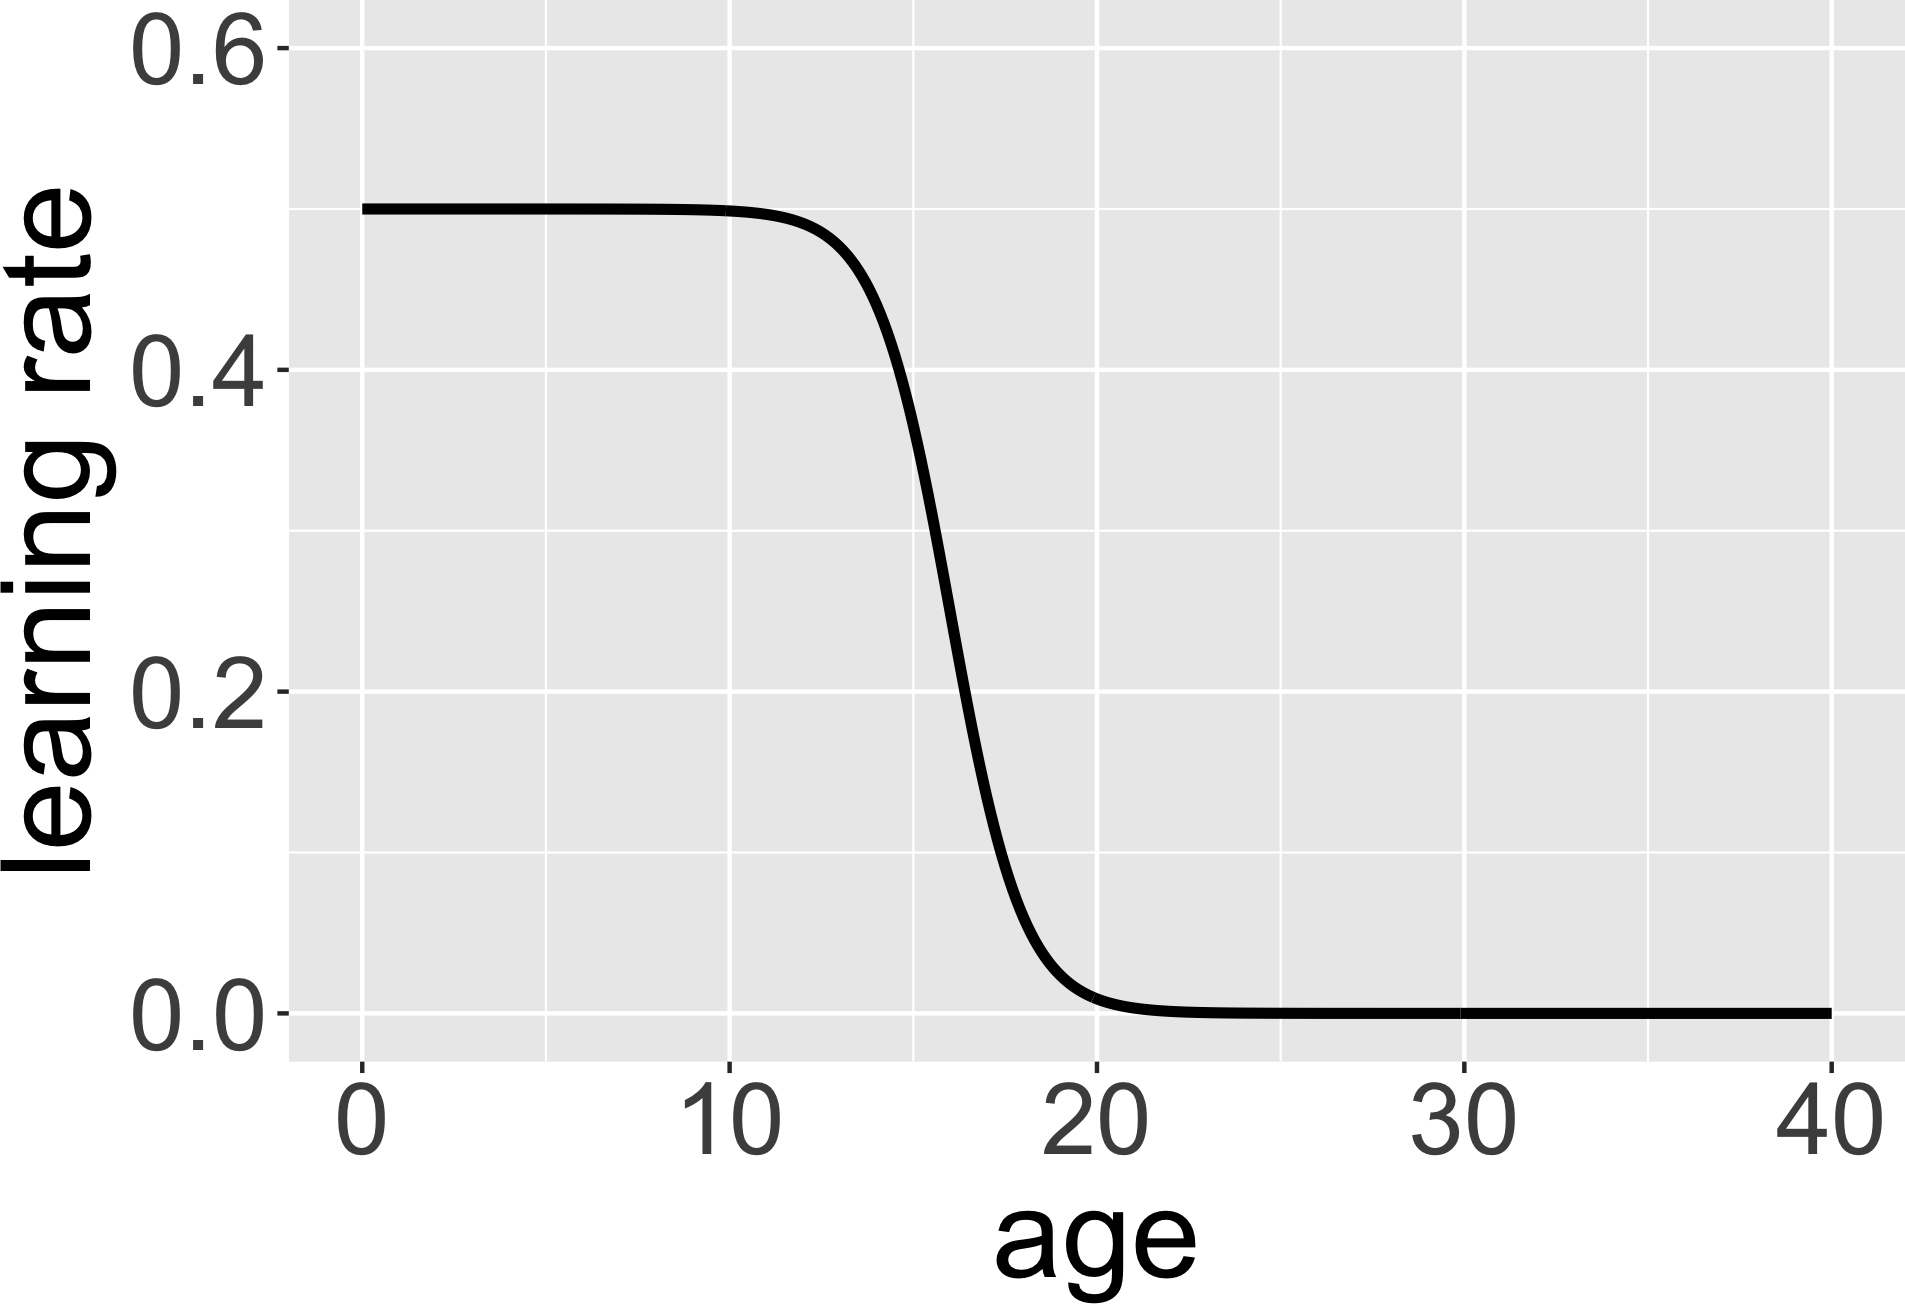
\includegraphics[width=0.24\linewidth]{SlikResponse_rmd_files/figure-latex/sigmoids-2} 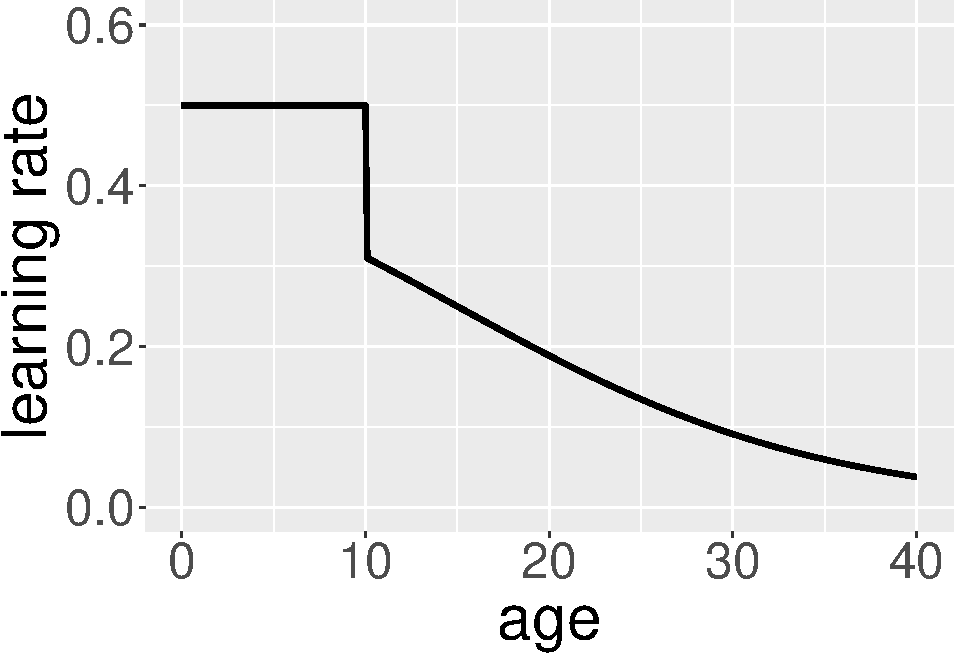
\includegraphics[width=0.24\linewidth]{SlikResponse_rmd_files/figure-latex/sigmoids-3} 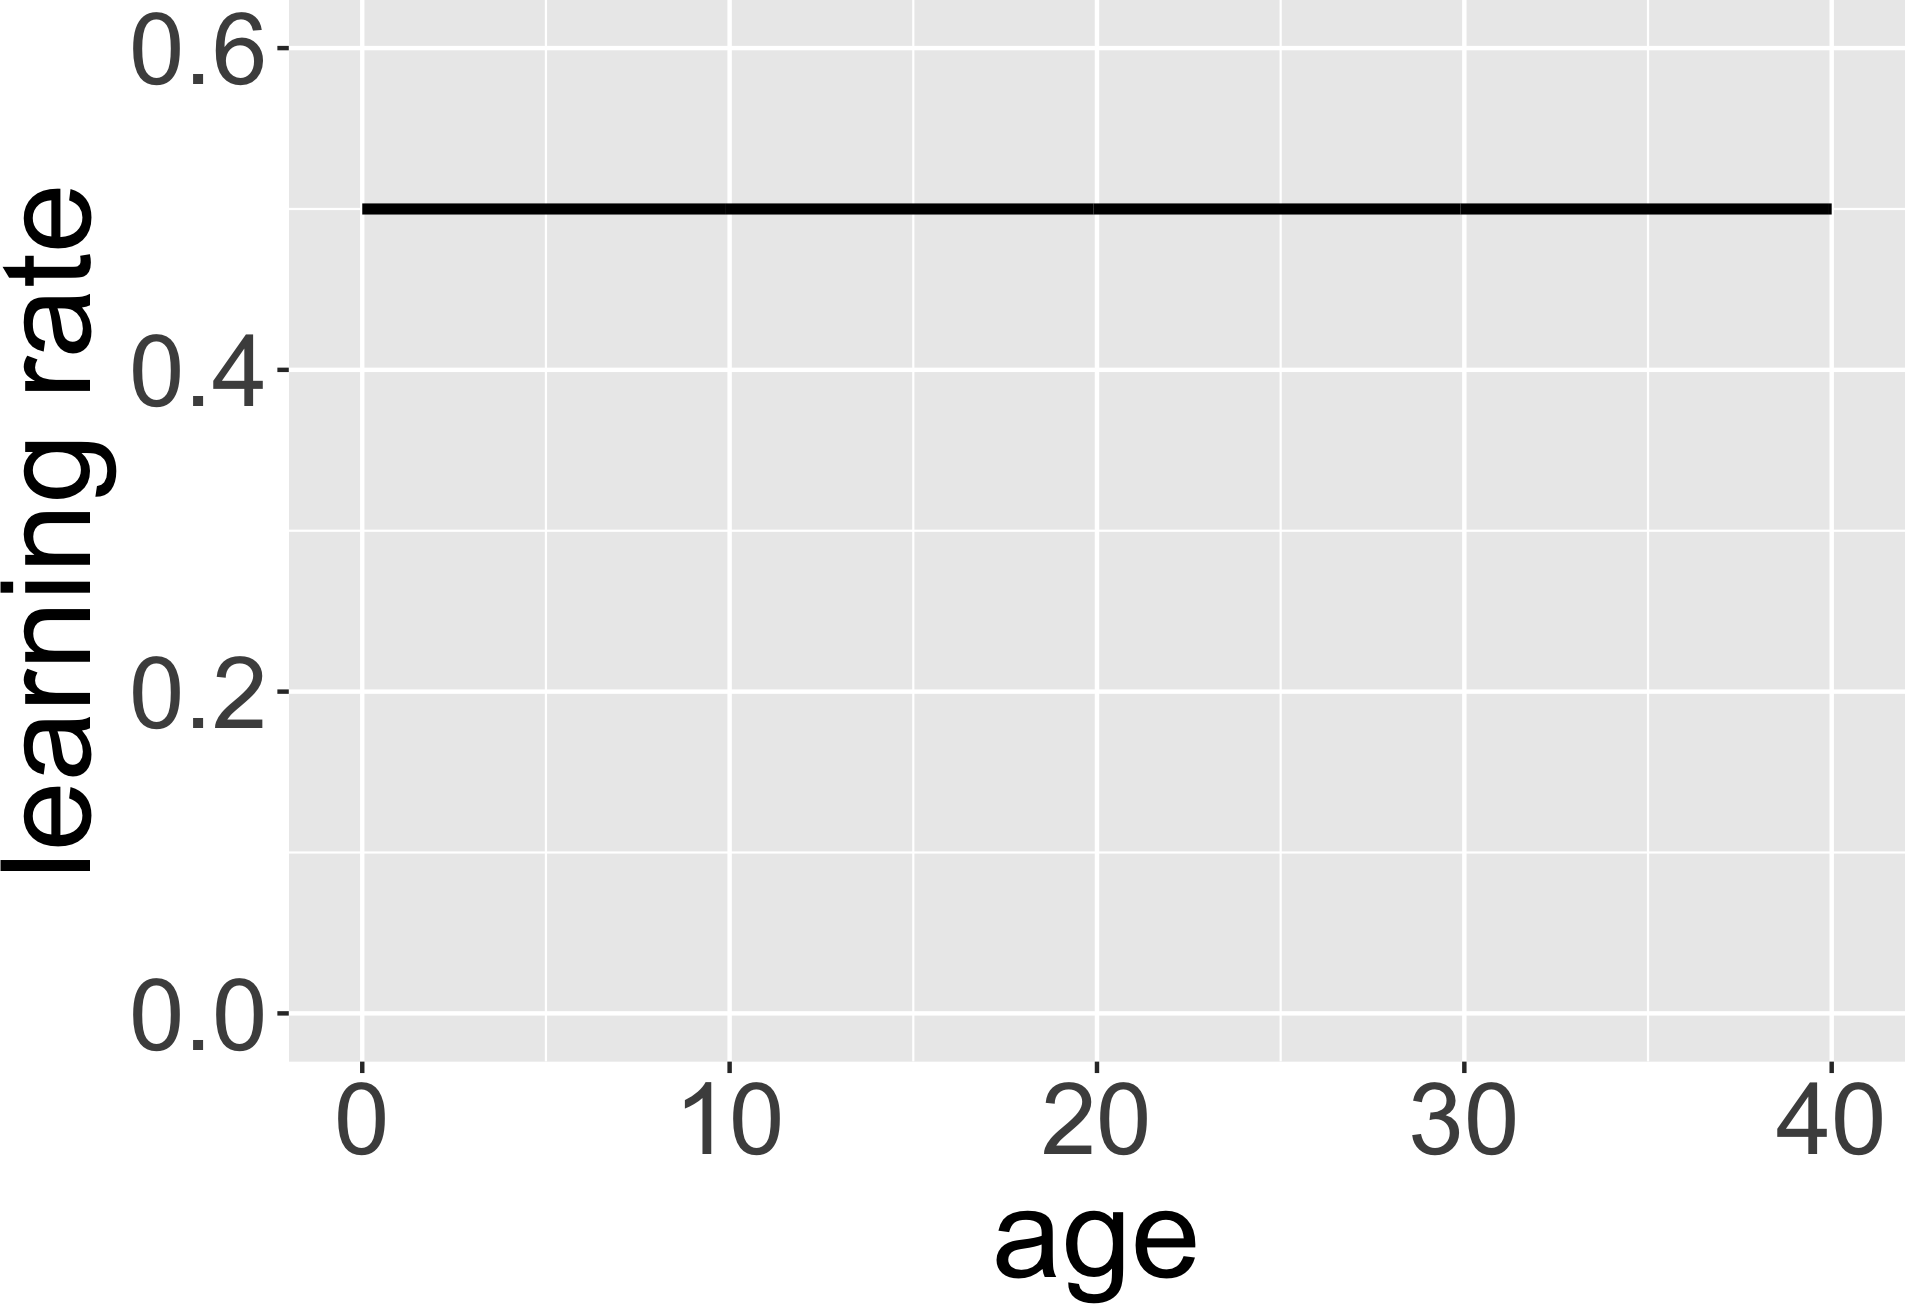
\includegraphics[width=0.24\linewidth]{SlikResponse_rmd_files/figure-latex/sigmoids-4} \caption{Examples of learning rate curves that could be inferred by HTP's model.}\label{fig:sigmoids}
\end{figure}

HTP's model had one final critical feature. They reasoned that bilinguals might learn English more slowly than monolinguals on account of having two languages to learn and thus less time to spend on each. HTP addressed this by allowing the effective learning rate for simultaneous bilinguals to be a percentage of the rate for monolinguals (the percentage was fit to the data). Similarly, individuals learning English in an immersion environment are expected to learn faster than those in a non-immersion environment, entirely independently of age. Again, HPT modeled these two groups as each learning at some percentage of the rate of monolinguals (these percentages were again fit to the data). HTP named this parameter \(E\) for ``Experience discount factor,'' on the intuition that it is capturing differences in the amount of input received by the four different groups. However, in practice it captures any fixed differences in the learning rates between the four groups (that is, differences that do not change with time).

Betraying a singular lack of creativity, HTP named the resulting model ``ELSD'', for ``Exponential Learning with Sigmoidal Decay.'' As already noted, it is a very simple model and makes a number of approximations and debatabler assumptions. However, the proof of the pudding is in the eating: the model captures key patterns in the data quite well (compare Fig. \ref{fig:HTP} A\&B with C\&D).

HTP investigated the consequences of critical aspects of the model by comparing to minimal alternatives. First, they compared the main results to those of a restricted version that assumes no decline in learning ability (\(r\)) with age. The best-fitting ``no-change'' model did not fit as well (\(R^2=66\)\% vs.~\(R^2=89\)\%). This poor fit is not surprising: if the no-change model fit well, the main model would have chosen a flat rate (cf.~Fig \ref{fig:sigmoids}). What this analysis does is help us better understand the consequences of not allowing learning rate to change with age. As shown in Fig. \ref{fig:HTP}C, the resulting model is able to capture the difference between monolinguals and simultaneous bilinguals (it does so through the \(E\) parameter). However, it cannot distinguish between later immersion learners, all of whom are (incorrectly) predicted to learn at the same rate regardless of the age at which they started. The same problem appears with non-immersion learners (Fig. \ref{fig:HTP}D).



\begin{figure}
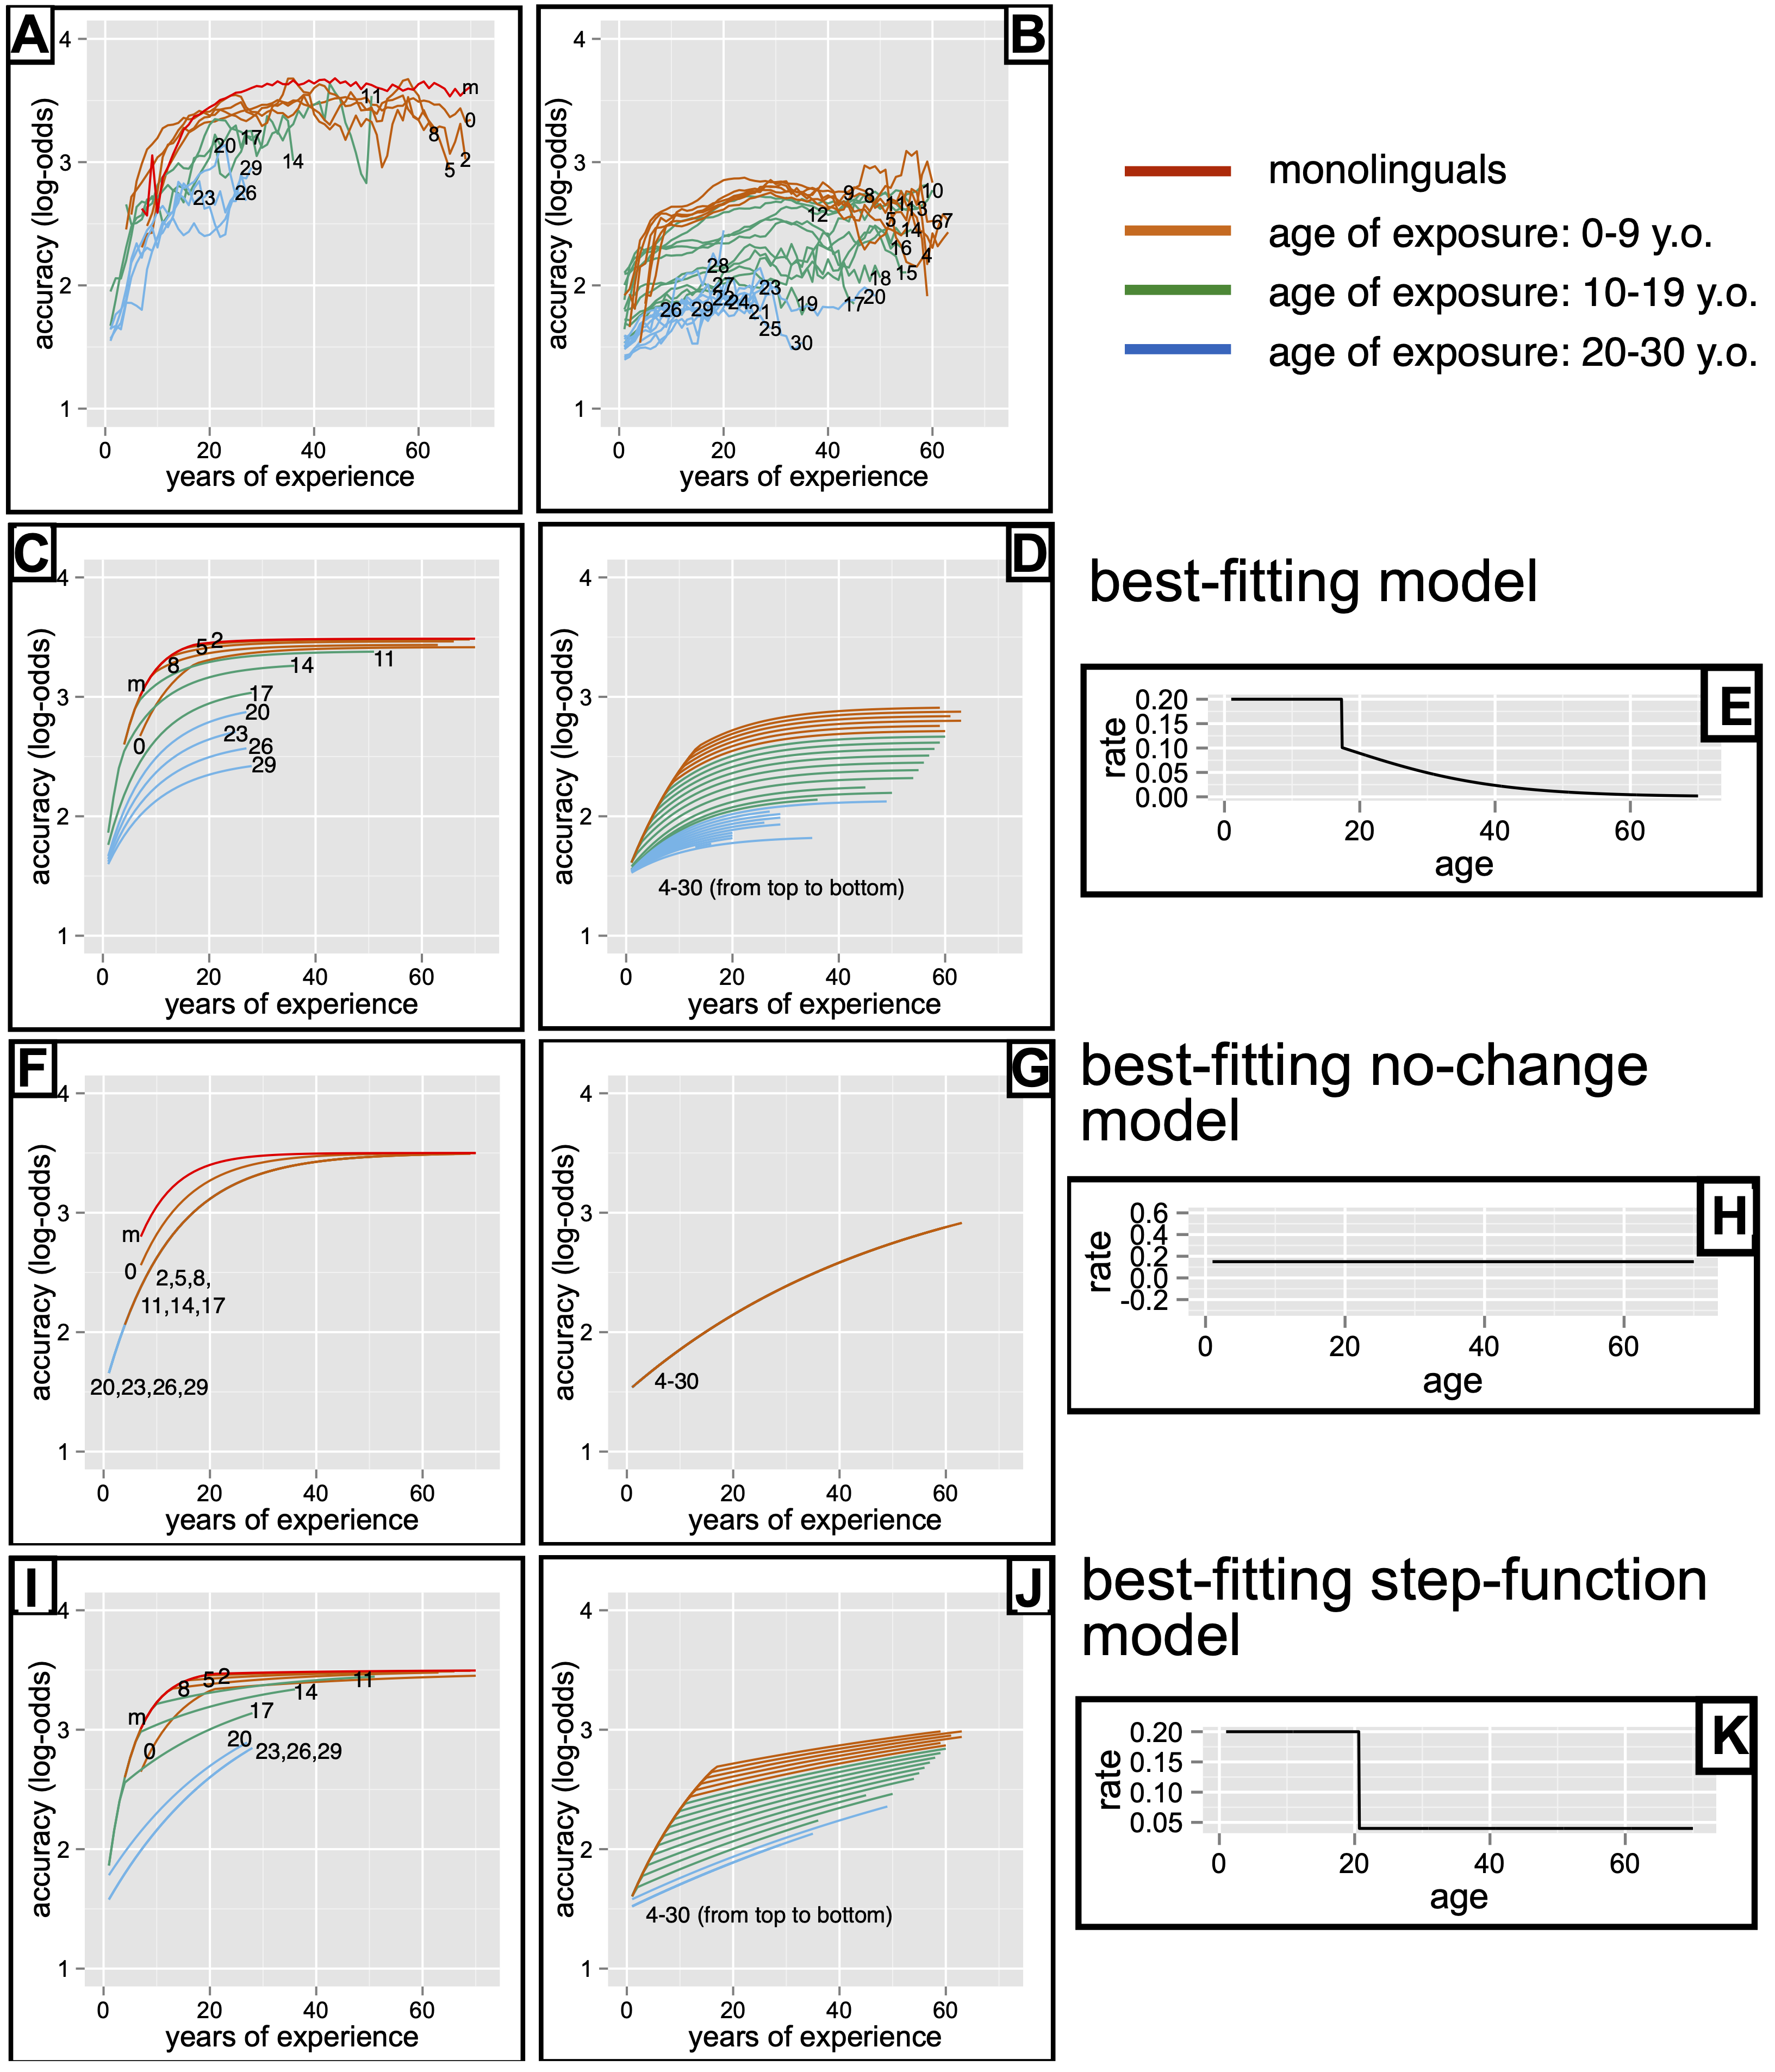
\includegraphics[width=1\linewidth,height=1\textheight]{Figures/Figure4} \caption{Figures from HTP, used with permission. Panels show the empirical results (top row), and the best fits for HTP's model (row 2nd from top) and two alternative models (bottom two rows). Monolinguals and immersion learners are plotted in the left panels (\emph{A}, \emph{C}, \emph{F}, \& \emph{I}). Non-immersion learners are shown in the middle column (\emph{B}, \emph{D}, \emph{G}, \& \emph{J}). In both the left and center columns, data/fits are plotted in terms of years of experience with the language, which makes the contrasts between models easier to see. Finally, panels in the right column show the models' estimated learning rate (\(r\)) as a function of age.}\label{fig:HTP}
\end{figure}

HTP also compared the main results to a variant that enforced a step-function from an early, higher learning rate (\(r_0\)) to a final, lower learning rate (\(r_1\)). The best-fitting step-function model fit less well (\(R^2\)=86\%; Fig. \ref{fig:HTP}K). The effect of positing that learning ability remains constant after the inferred critical age is to diminish differences among later learners. This is most clearly evident in learners who begin after the critical age, who are indistinguishable (compare: \ref{fig:HTP}I \& C).\footnote{A third variant, which assumed learning rate changed with years of experience rather than age, is not immediately relevant to the present conversation. For details, see HTP Supplementary Materials.}

HTP report a large number of additional results, including follow-up analyses, manipulation checks, and statistical power simulations. For these, we refer the reader to the original manuscript.

\hypertarget{reanalysis-by-van-der-slik-schepens-bongaerts-and-van-hout-2021-ssbh}{%
\section{Reanalysis by van der Slik, Schepens, Bongaerts, and van Hout (2021) (SSBH)}\label{reanalysis-by-van-der-slik-schepens-bongaerts-and-van-hout-2021-ssbh}}

Recently, Slik, Schepens, Bongaerts, and Hout (2021) (henceforth, \emph{SSBH}) took issue with the analyses described above and proposed alternatives that, they assert, provide different results.

Many of the concerns they raise involve misconceptions, misreadings, and miscalculations. For instance, they ``fail to reproduce'' some of HTP's results by virtue of failing to follow key steps in the analyses. In one example, SSBH note that they are unable to reproduce the number of subjects after exclusions. This turns out to be due to the fact they use different exclusions. Similarly, they report they obtain higher \(R^2\) values for some key model fits. On inspection, this is revealed to be a consequence of not using cross-validation; the consequence is an inflated \(R^2\). They express worry about HTP's data quality, on account of HTP supposedly needing to exclude over 100,000 subjects (\textgreater{}\(\frac{1}{7}\)) due to missing data. In fact, these subjects were not included because they were non-native speakers of English whose linguistic histories involved a mixture of immersion and non-immersion learning, thus not meeting the definitions of either category. This confusion seems to stem from SSBH's misreading of the learner group definitions, which they misquote in their own manuscript.

I have included an extensive list of these and other corrections in the Appendix. In the main manuscript, I focus on SSBH's core contention: HTP's observation of a rapid decline in language learning at 17-18 years old is due entirely to specific subsets of the subjects (namely non-immersion learners and later immersion learners). The question of whether age affects different learner groups differently is of broad theoretical interest and at the heart of both HTP and SSBH. Below, I first show that SSBH's findings derive from miscalculations, illogics, and a failure to consider statistical significance. However, the question remains interesting, and so I then present an updated version of their analyses, drawing on more recent work Chen \& Hartshorne (2021). These results strongly support HTP's original findings. I conclude by discussing remaining open questions and possible next steps.

\hypertarget{do-all-learner-groups-show-a-rapid-decline-in-late-adolescence-ssbhs-analyses}{%
\subsection{Do All Learner Groups Show a Rapid Decline in Late Adolescence? SSBH's Analyses}\label{do-all-learner-groups-show-a-rapid-decline-in-late-adolescence-ssbhs-analyses}}

\hypertarget{discontinuous-vs.-continuous-models}{%
\subsubsection{Discontinuous vs.~``Continuous'' Models}\label{discontinuous-vs.-continuous-models}}

SSBH state that their first ``main objection'' is that:

\begin{quote}
\emph{HTP defined a continuous learning rate model (see their figure S2, p.~2; S indicates Supplementary Information), but they did not report any outcomes for this model. The occurrence of a discontinuity is a crucial argument in their positive evaluation of the critical period hypothesis. A proper evaluation includes, in our view, comparing the fit of a continuous model with the fit of a discontinuous model.} (p.~3)
\end{quote}

SSBH highlight two primary concerns. Their first is that:

\begin{quote}
\emph{HTP defined a continuous learning rate model (see their figure S2, p.~2; S indicates Supplementary Information), but they did not report any outcomes for this model. The occurrence of a discontinuity is a crucial argument in their positive evaluation of the critical period hypothesis. A proper evaluation includes, in our view, comparing the fit of a continuous model with the fit of a discontinuous model.}
\hfill --- SSBH, p.~3
\end{quote}

This statement is predicated on a factual error and a conceptual error. The figure they reference, as explained in its caption, depicts six examples of learning rate curves recoverable by the ELSD model -- including the possibility of no discontinuity (see also Fig. \ref{fig:sigmoids}). Indeed, this should be obvious from the fact that their ``alternative'' model is in fact the ELSD model with the critical age parameter (\(t_c\)) fixed at 1 -- or sometimes fixed at 0; SSBH give no explanation for varying this parameter across analyses. Thus, as a factual matter, HTP did in fact consider SSBH's ``continuous'' model and rejected it because it did not fit as well.

SSBH, however, suggest a different statistical test: Rather than fitting a single overarching model, they separately fit the full ELSD model and their restricted ELSD model (their ``continuous'' model), and compare the best fits for the two models using Akaike's Information Criterion {[}AIC; Akaike (1974){]}. This is a more conservative test, since AIC penalizes the full ELSD model for having one additional free parameter: \(t_c\). That is, since more complex models generally fit the data better, AIC asks whether the the full ELSD model improves the fit enough to justify a more complex model (that is, the inclusion of the free parameter \(t_c\)).

Critically, asking whether the free parameter \(t_c\) is justified answers a very different question from the one SSBH asked: does the data justify a discontinuity in learning rate? By definition, what SSBH call the ``discontinuous'' model (the one with \(t_c\) as a free parameter) can fit anything their ``continuous'' model (the one with \(t_c\) fixed to 0 or 1) can fit, including rapid age-related declines, gradual age-related declines, or no age-related decline at all. As I reviewed above, the real difference is that the ``continuous'' model can only infer \emph{symmetric} declines; it cannot accommodate declines that start rapidly and then slow down, nor those that start slowly and then continue to gather speed. The full ELSD model uses the \(t_c\) parameter to approximate an asymmetric sigmoid with an initially rapid decline that then slows down. (Neither model allows for a decline that only gains speed over time; this limitation was addressed by Chen and Hartshorne (2021).)

The initial decline inferred by the ELSD model can be quite steep, but this is a limitation of the mathematical approximation, not a theoretical claim. Clearly, nobody thinks that all people lose half their ability to learn language overnight, exactly when they turn 17.4. In any case, the best way to test whether the decline is asymmetric and instantaneous as opposed to asymmetric and merely very rapid would be to identify a model that allows for a smoother asymmetry. For just such an analysis, see Chen and Hartshorne (2021) and also below.

Since HTP already established that an asymmetric decline fits the data substantially better than a symmetric one, SSBH's analyses amount to asking whether this improved fit is enough to justify the additional free parameter. In fact, as SSBH report, it does (SSBH, Table 1 and surrounding text). In short, SSBH's own analyses militate against their first main objection. Nonetheless, SSBH state the the outcome is ``inconclusive'', because ``although mathematically the {[}full ELSD{]} model appears to the be best, there are logical reasons to prefer the continuous {[}model{]}'' (pp.~10-11). Specifically, they believe that a sharp drop in learning ability -- as inferred by the full ELSD model -- is \emph{a priori} unlikely, as is the relatively high initial learning rate for immersion learners. The second point is based on a misreading of the literature: as I reviewed above, it is established that the initial learning rate for immersion learners \emph{exceeds} that of monolinguals (Snow \& Hoefnagel-Höhle, 1978).

I am actually sympathetic to their first point: the Bayesian perspective that \emph{a priori} unlikely hypotheses should be dispreferred. This is often glossed as ``extraordinary claims require extraordinary evidence.'' How extraordinary is the evidence here? The AIC-adjusted relative likelihood of the best-fitting full ELSD model is 10\^{}159 (SSBH report it as ``\(>10^5\)'', which substantiall understates the difference). Even using the Bayesian Information Criterion (BIC), which is far more biased against complex models than is AIC (Wagenmakers, 2007), the full ELSD model is 10\^{}157 times more probable than SSBH's ``continuous'' model. By any definition, this constitutes extraordinary evidence. Following standard Bayesian calculations, even if the ``continuous'' model was \emph{a priori} a trillion times more likely than the full ELSD model, the posterior probability given the data would still favor the full ELSD model by a factor of 10\^{}145 to 1. Thus, by any measure, in this contest between empirical data and \emph{a priori} assumptions, the data win this round.

Instead, SSBH reject the results of their test of their hypothesis and propose a new test.

\hypertarget{separate-investigation-of-different-learner-groups}{%
\subsubsection{Separate investigation of different learner groups}\label{separate-investigation-of-different-learner-groups}}

SSBH state that their second main objection is that HTP analyzed all subjects with a single model, rather than separately analyzing different learner groups: monolinguals, simultaneous bilinguals, non-immersion bilinguals, etc. They hypothesize that the model will not infer a sharply-defined critical period for every group. Once again, they operationalize this hypothesis as a prediction that their ``continuous'' model will fit better than the full ELSD model, using AIC-based comparison. They report that the ``continuous'' model is indeed preferred for native speakers (both monolinguals and simultaneous bilinguals), but not for immersion learners or non-immersion learners. They then reject the results for the immersion learners and separately analyzing immersion learners who began before the age of 10, this time finding a better fit for the ``continuous'' model (the results for immersion learners who began at the age of 10 or later remain the same).

These conclusions are mistaken. As I explain below, their operationalization of their hypothesis is based on a logical fallacy, and their results are not statistically significant -- and even if the results were statistically significant, they actually confirm rather than contradict HTP's results.

\hypertarget{operationalizing-the-ssbh-hypothesis}{%
\paragraph{Operationalizing the SSBH Hypothesis}\label{operationalizing-the-ssbh-hypothesis}}

SSBH's key conceptual error is neglecting the fact that we expect learners' pace of learning to decline over time. As explained above, the pace of learning inevitably declines as learners run out of easy, high-frequency constructions to learn. This is of course not just a feature of language learning but a feature of doing just about anything and epitomized in the famous 80/20 rule: 80\% of any project can be accomplished in the first 20\% of the time.

As discussed above, later learners' pace of learning is slower than that of monolinguals (see Fig. \ref{fig:sigmoids}, right). The goal of both the full ELSD model and the ``continuous'' model is to determine how much of this difference can be explained by allowing the decay (``learning'') rate to change with age. That is, these models ask, ``What sort of age-related decline in learning could account for later learners under-performing native speaker norms?'' Obviously, there is no way to ask this question about monolinguals themselves (e.g., What sort of age-related decline in learning could account for monolinguals under-performing monolingual norms?``) or about simultaneous bilinguals (''What sort of age-related decline in learning could account for simultaneous bilinguals under-performing simultaneous bilingual norms?{}``).

In short, native language acquisition fully confounds two causes of the diminishing pace of learning: age-related decline in ability and simply running out of things to learn. Because older learners also have less left to learn, it is impossible to determine how much the decline in observed learning is due to age and how much is due to having less to learn. To tease these causes apart, we must deconfound them: for instance, by comparing people who started learning the language at different ages. Indeed, it is the existence of late learners (and their difficulties learning) that spurred research into critical periods for language. In a counterfactual world where there were no second-language learners (or late first-language learners), the question of critical periods would probably never have arisen. By analogy, the fact that everyone alive today learned to breath at birth is probably related to the singular dearth of research into critical periods for learning to breath. The ELSD model exploits these differences betweeen early and late learners to try to estimate the effect of age.

Thus, many of SSBH's analyses end up asking a different question: does the learning curve for individuals all of whom began learning English at the same age depart from a perfect exponential decay function in a way that can be explained by an age-related decline in the decay (``learning'') rate? If we knew for sure that in the absence of age-related decline, learning curves would perfectly follow exponential decay, asking that question would be meaningful. However, we don't know that and it probably isn't true. At a minimum, there are other influences on the pace of learning, such as entry into (or exit from) formal education, which also influence learning curves and make it harder to isolate the independent effects of age. To make matters worse, inspection of the raw learning curves indicates that any age-related change must occur somewhere between mid-adolescence and early adulthood (see discussion above) -- a time at which native speakers are already fairly close to ceiling. Thus, any age-related changes that occur that late will have only subtle impacts on native speaker learning curves, making the impact of age-related changes difficult to detect (see Fig. \ref{fig:latechanges}). Effects this small are likely to be swamped by statistical noise or other sources of variation in the data.

In short, whatever one thinks of SSBH's hypothesis that different learners groups are affected differently by age, their method of testing the hypothesis was not well-suited to the problem.



\begin{figure}
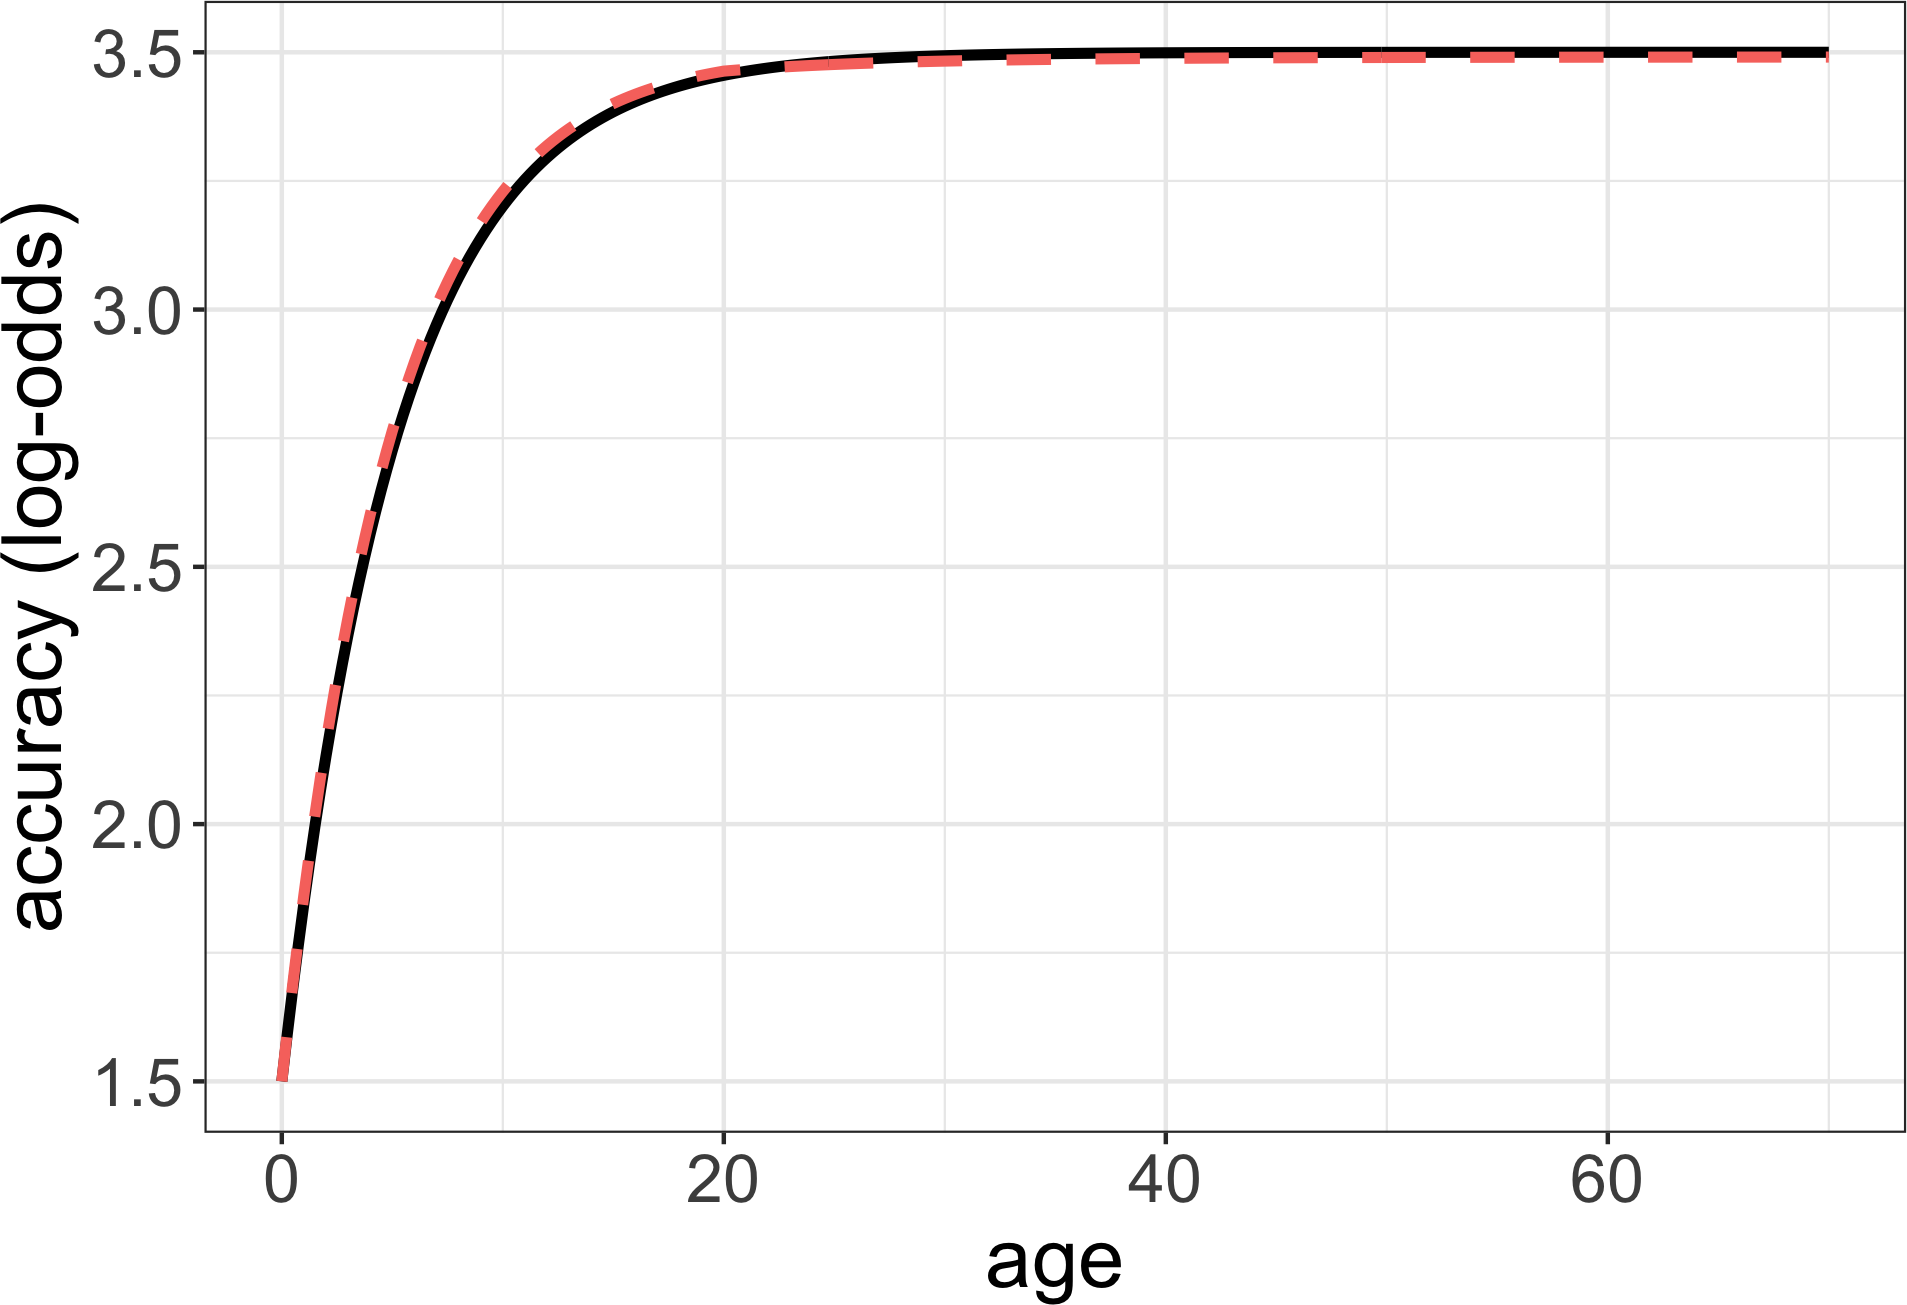
\includegraphics[width=0.35\linewidth]{SlikResponse_rmd_files/figure-latex/latechanges-1} \caption{Examples of learning rate curves that could be inferred by HTP's model.}\label{fig:latechanges}
\end{figure}

\hypertarget{lack-of-statistical-significance}{%
\paragraph{Lack of Statistical Significance}\label{lack-of-statistical-significance}}



\begin{figure}
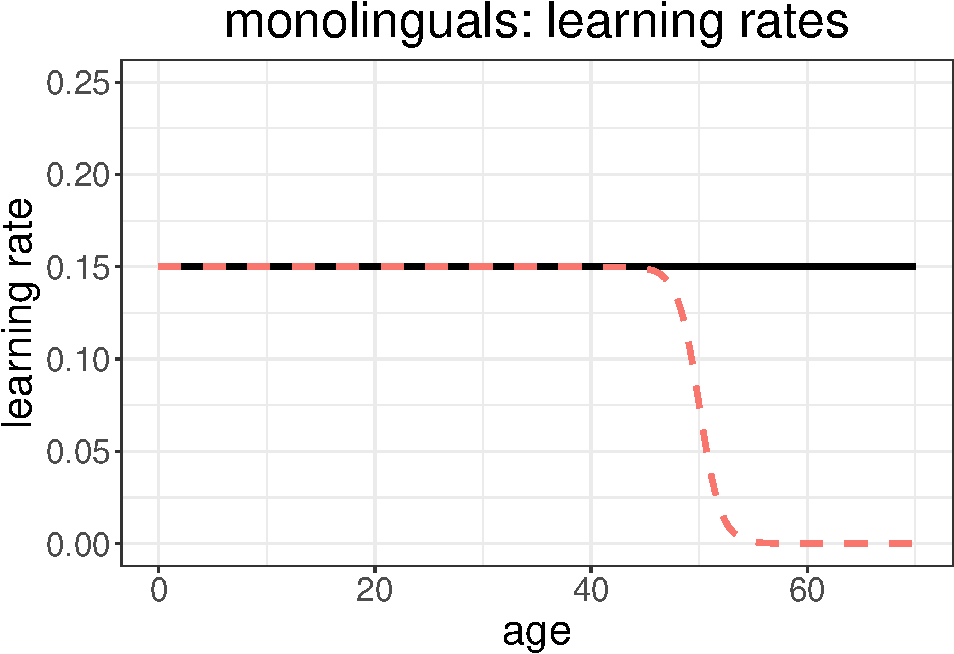
\includegraphics[width=0.48\linewidth]{SlikResponse_rmd_files/figure-latex/natives-1} 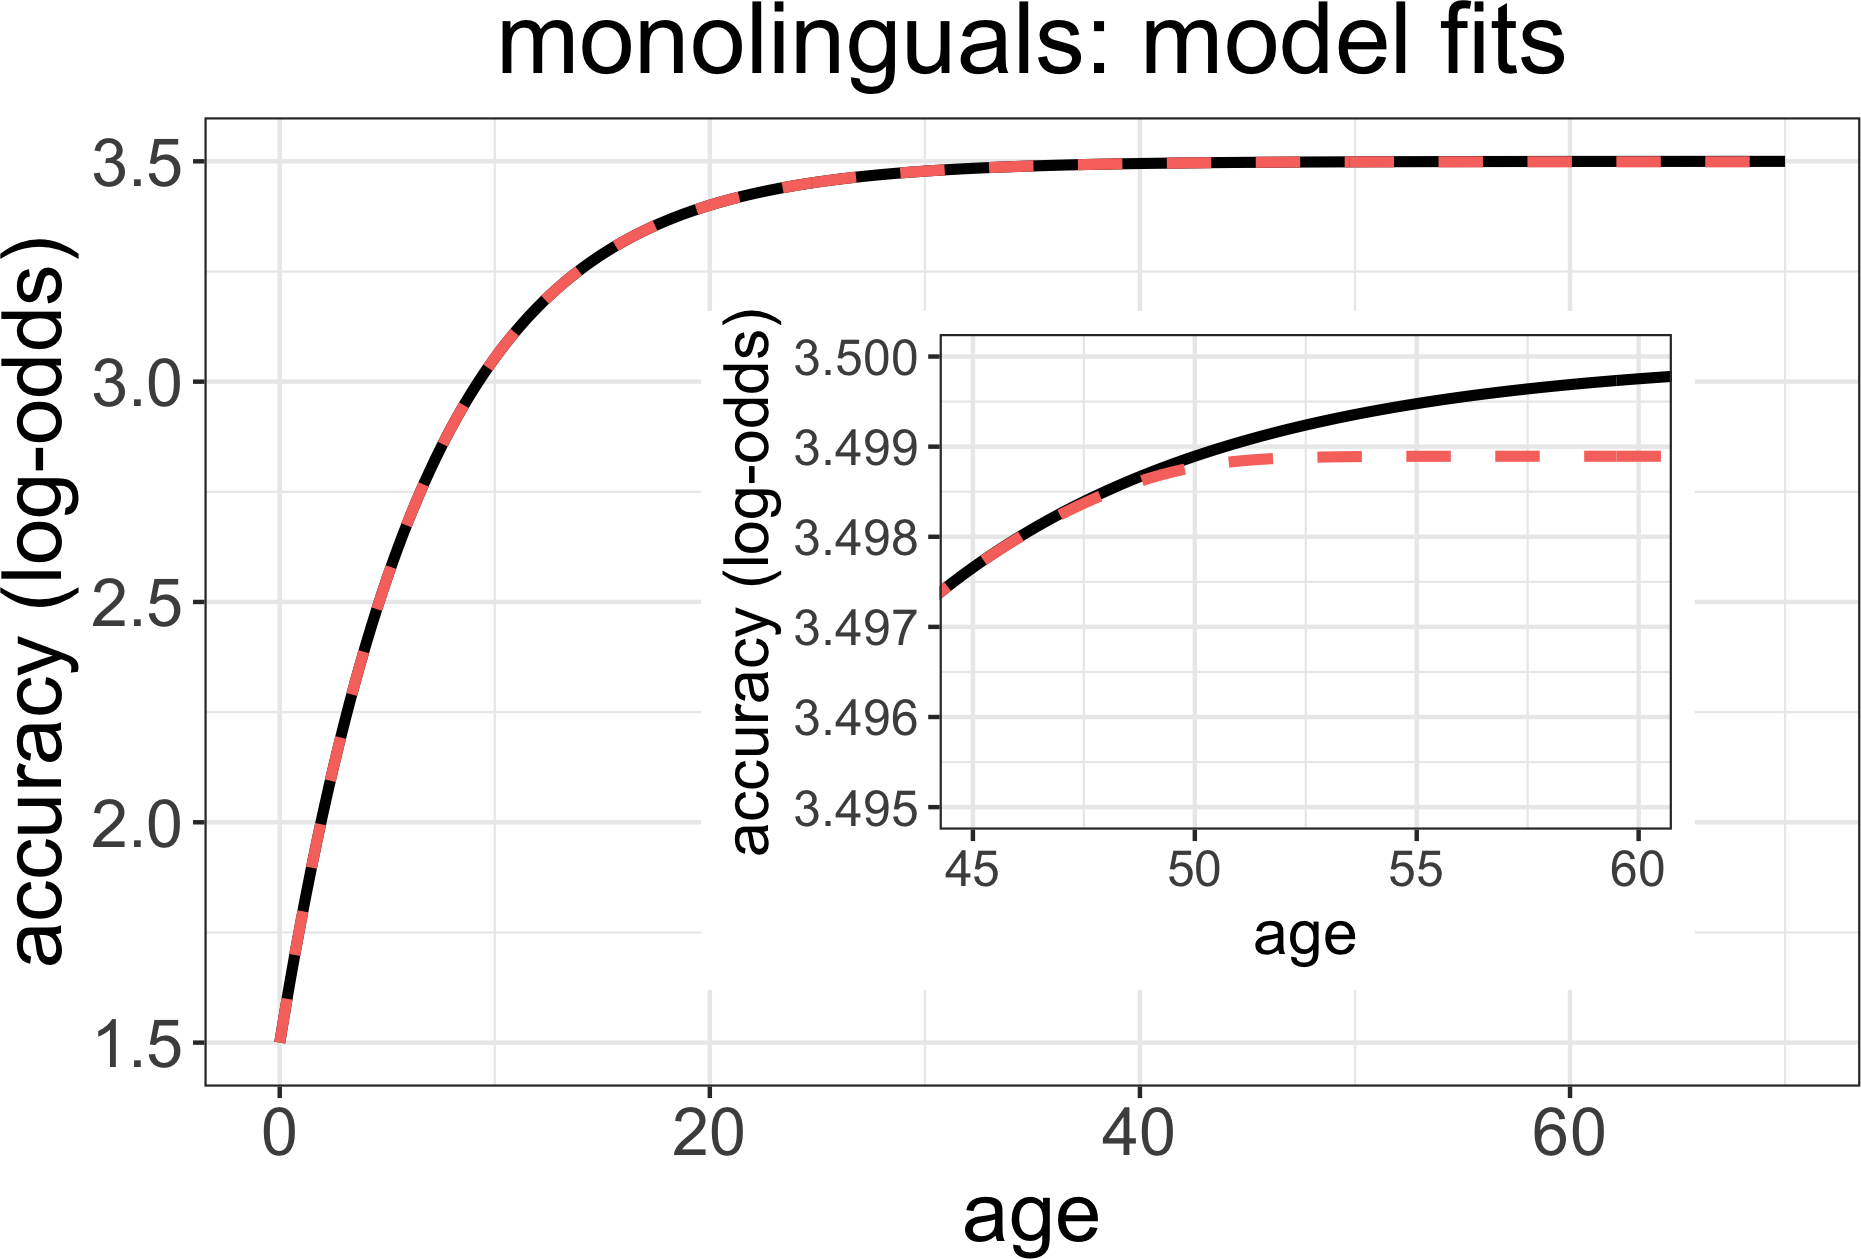
\includegraphics[width=0.48\linewidth]{SlikResponse_rmd_files/figure-latex/natives-2} 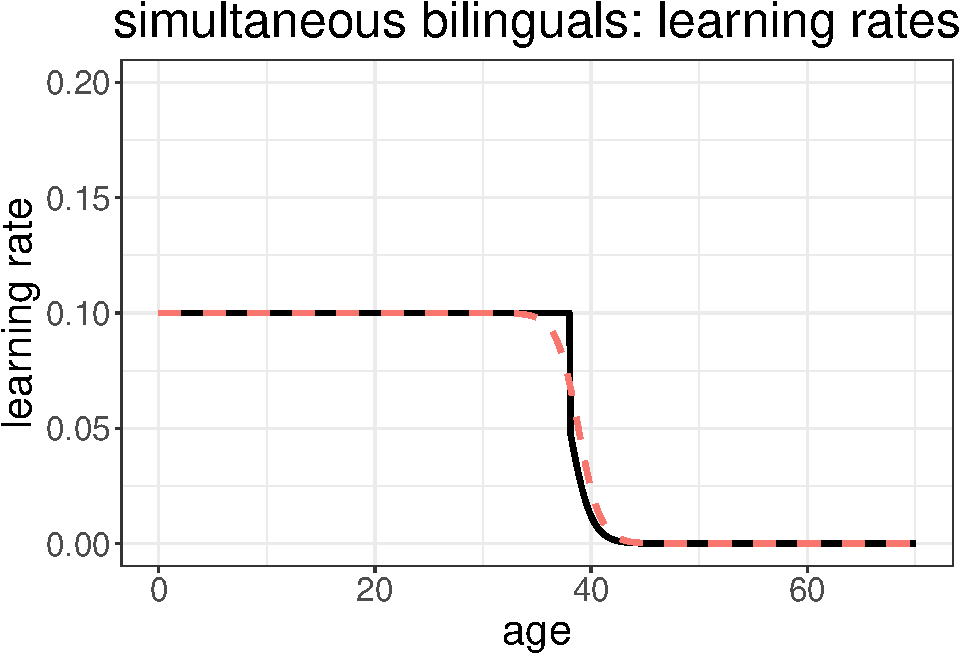
\includegraphics[width=0.48\linewidth]{SlikResponse_rmd_files/figure-latex/natives-3} 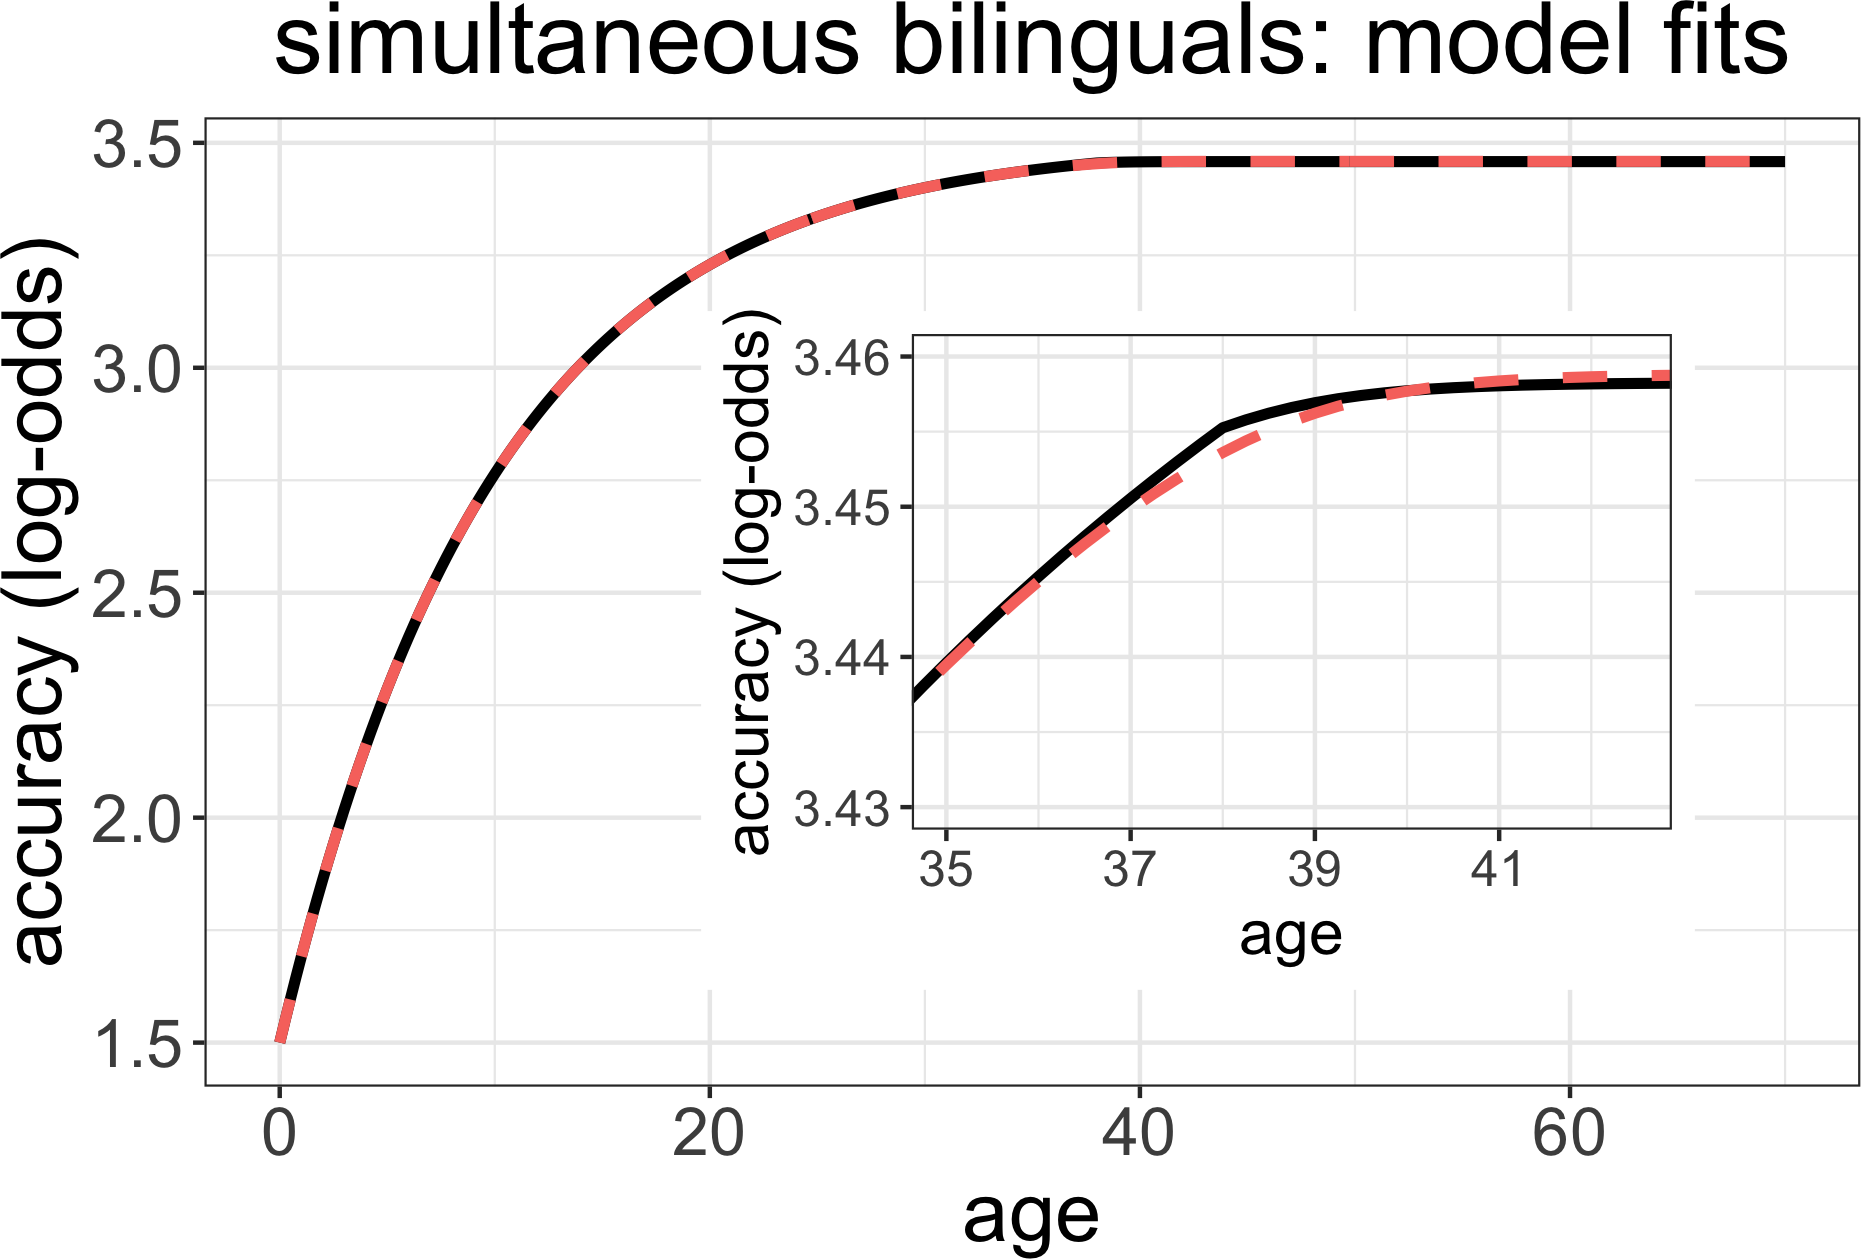
\includegraphics[width=0.48\linewidth]{SlikResponse_rmd_files/figure-latex/natives-4} \caption{SSBH analyzed each learner group separately. Inferred age-related changes in learning curves (\emph{left panels}) and model fits (\emph{right panels}) for monolinguals only (\emph{top panels}) and simultaneous bilinguals only (\emph{bottom panels}). \emph{Solid black}: HTP's ELSD model. \emph{Dashed red}: SSBH's continuous model.}\label{fig:natives}
\end{figure}

Even if one accepts SSBH's reasoning, there is a further problem: their results are not statistically significant. AIC values are not directly interpretable, only their differences are. In every case where SSBH report an analysis that favors their ``continuous'' model, the difference in AIC is less than 2, less than half the conventional threshold for reaching significance (Burnham \& Anderson, 1998). For instance, the full ELSD model actually fits the monolingual data slightly better than the ``continuous'' model (log-likelihood = 45.90 vs.~45.80, respectively), but because the full model has one extra parameter, the AIC analysis slightly prefers the ``continuous'' model (\$AIC\_diff = \(1.90). (As described in the Appendix, SSBH miscalculate AIC, so I use the corrected numbers here. However, the results are not significant even using their numbers.) For the simultaneous bilinguals, the full ELSD model fits slightly worse than the "continuous" model both in terms of (log-likelihood = 70.70 vs. 71.30 and AIC (\)AIC\_diff = \(2.60), but the difference is again well below the threshold for significance. The final analysis that SSBH claim supports the "continuous" model involves immersion learners who began before the age of 10. As with monolinguals, the full ELSD model actually fits the data a bit better than the "continuous" model (log-likelihood = 112.90 vs. 112.90, and while the AIC difference is slightly in the direction of the "continuous" model, it does not reach significance (\)AIC\_diff = \$1.90).

Note that in contrast, every analysis reported by SSBH that supports the full ELSD model supports it at essentially ceiling levels.

\hypertarget{a-distinction-without-a-difference}{%
\paragraph{A Distinction without a Difference}\label{a-distinction-without-a-difference}}

Leaving aside whether the analyses make sense or are significant, a further problem for SSBH is that they focus on which model provides a better fit, largely ignoring the fits themselves. In every case where the ``continuous'' model achieves a slightly better AIC, the fits of the two models are essentially identical. For monolinguals, SSBH note that the full ELSD model finds no age-related change in learning at all (Fig. \ref{fig:natives}, top left), while the continuous model finds a decline at around 50 years old (under the optimization parameters used by SSBH, the continuous model -- but not the full ELSD model -- \emph{must} have a decline somewhere before the age of 50). However, since under both models learners have essentially reach asymptote by the age of 30, so changes in the learning rate at the age of 50 do not make a detectable difference. Indeed, the model fits for the full ELSD model and the continuous model are distinguishable only under \emph{extremely} high magnification(Fig. \ref{fig:natives}, top right; note scale on inset). SSBH's results for simultaneous bilinguals are similar: both models infer essentially the same sharp drop in learning ability in the late 30s. The drop is slightly sharper for the full ELSD model (Fig. \ref{fig:natives}, bottom left), but because the drop happens when learners are already near ceiling, this is a distinction with a difference only observable under extremely high magnification (see Fig. \ref{fig:natives}, bottom right, and insert). The differences between the models for immersion learners who began before the age of 10 as similarly unimpressive (Fig. \ref{fig:immersion}, top right). By contrast, the models do make different predictions for late immersion learners, but as reported by SSBH, these analyses strongly favor the full ELSD model (see Fig. \ref{fig:immersion}, bottom.)

To summarize so far, the comparison of the full ELSD and ``continuous'' models is based on a misunderstanding, and in every case either the results strongly support the full ELSD model or the two models do not give statistically or substantively different results.



\begin{figure}
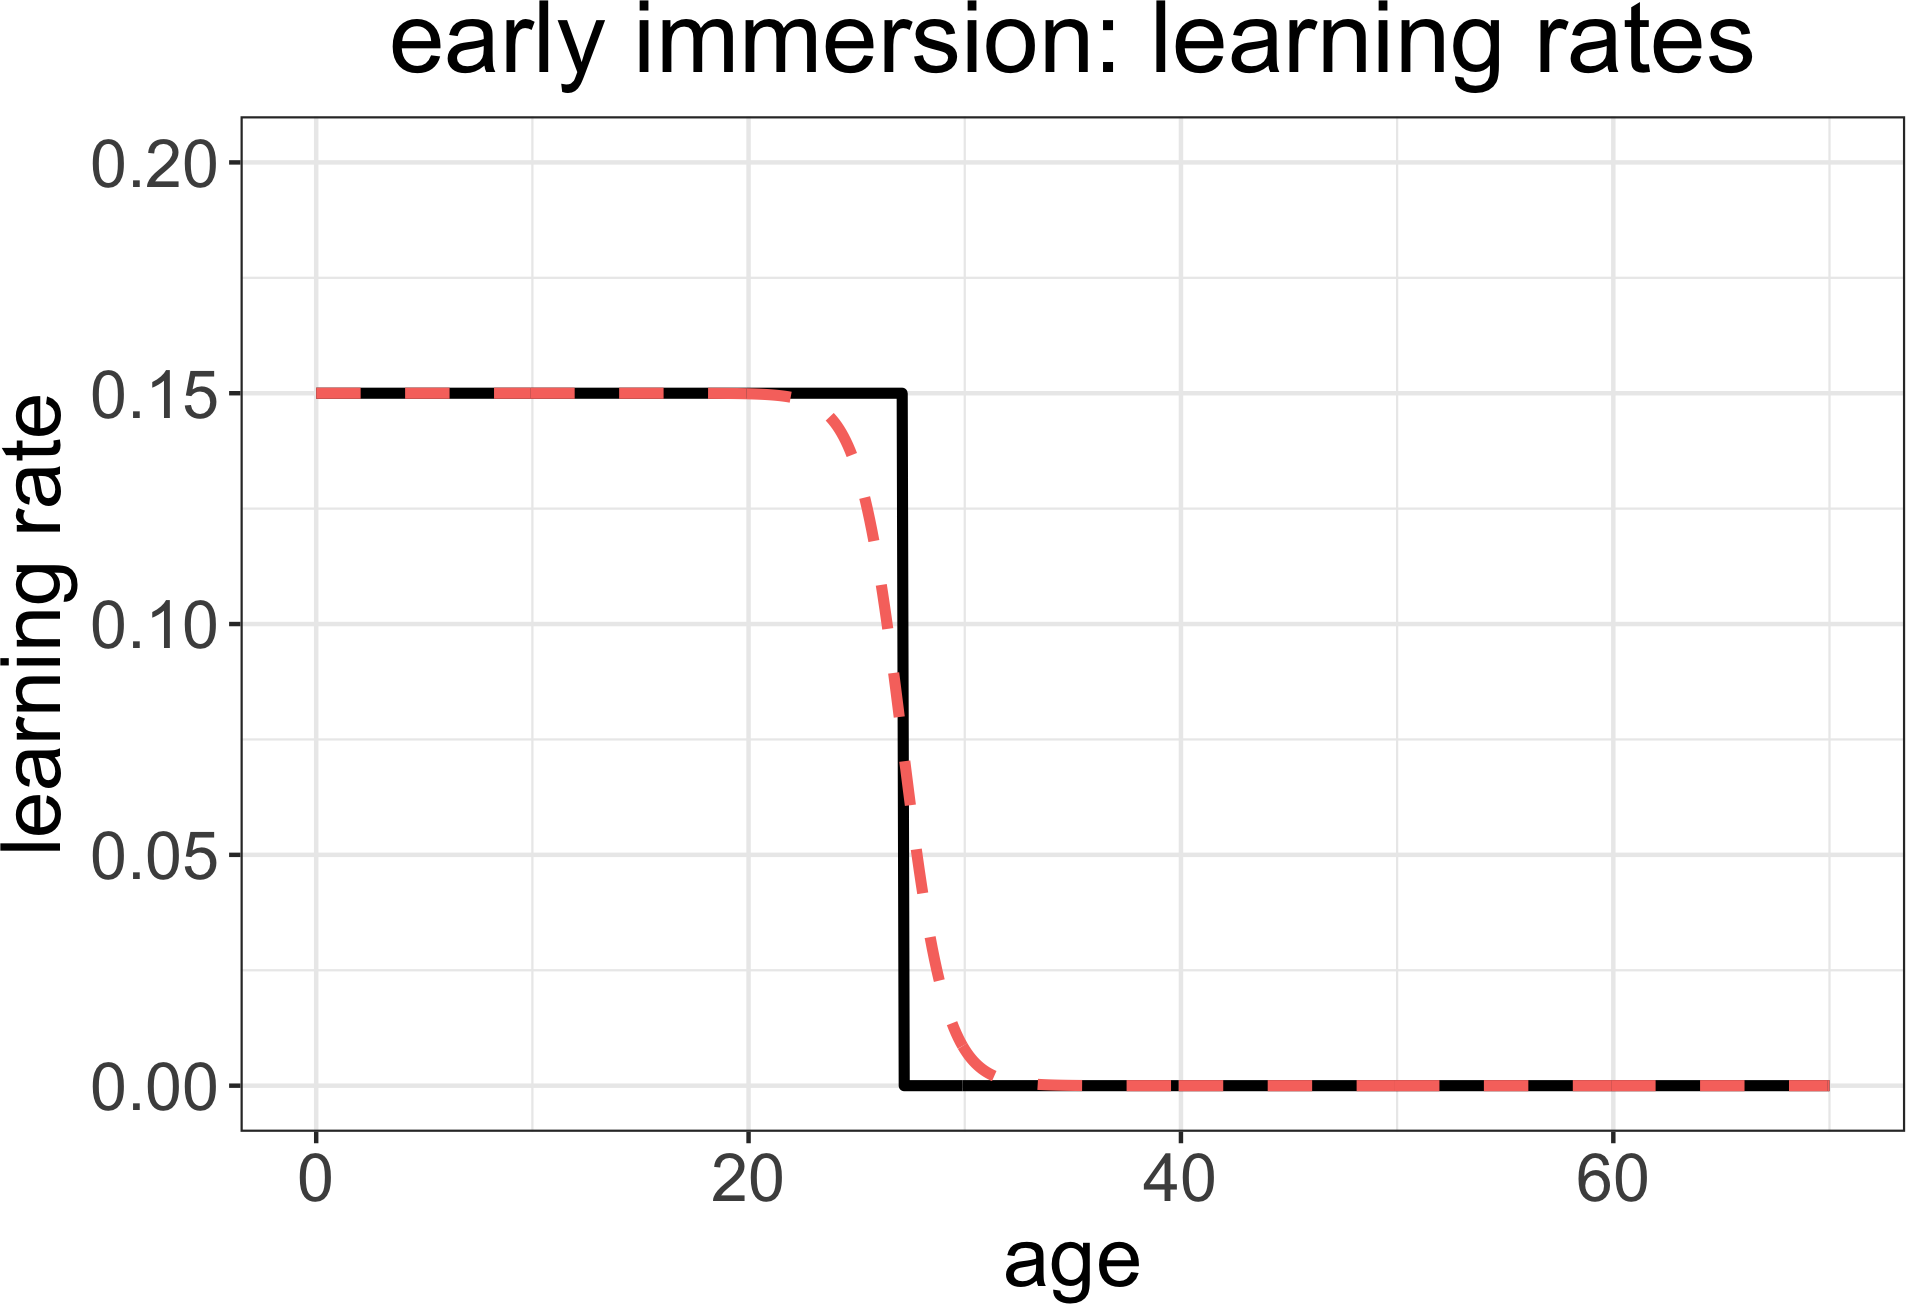
\includegraphics[width=0.48\linewidth]{SlikResponse_rmd_files/figure-latex/immersion-1} 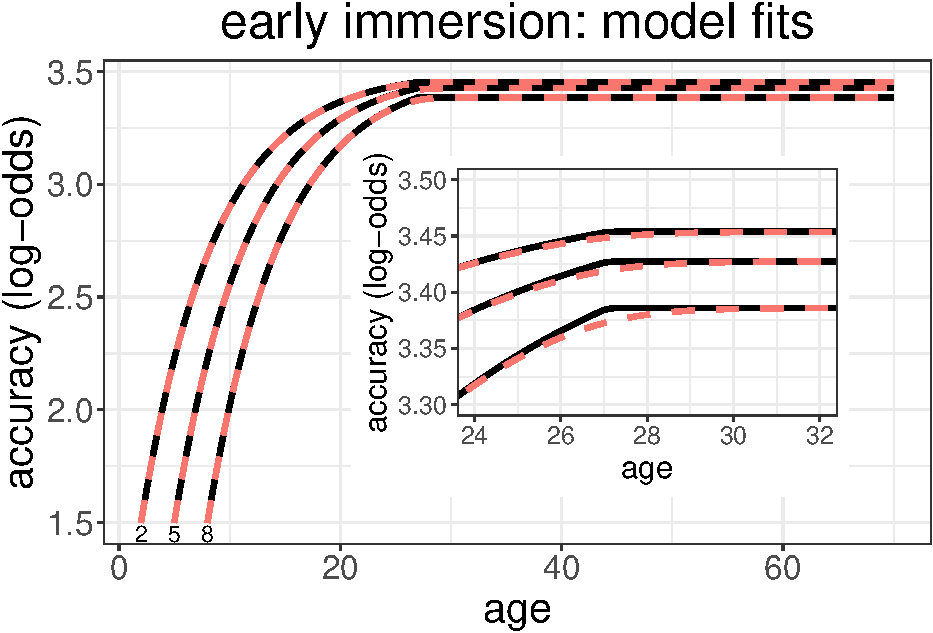
\includegraphics[width=0.48\linewidth]{SlikResponse_rmd_files/figure-latex/immersion-2} 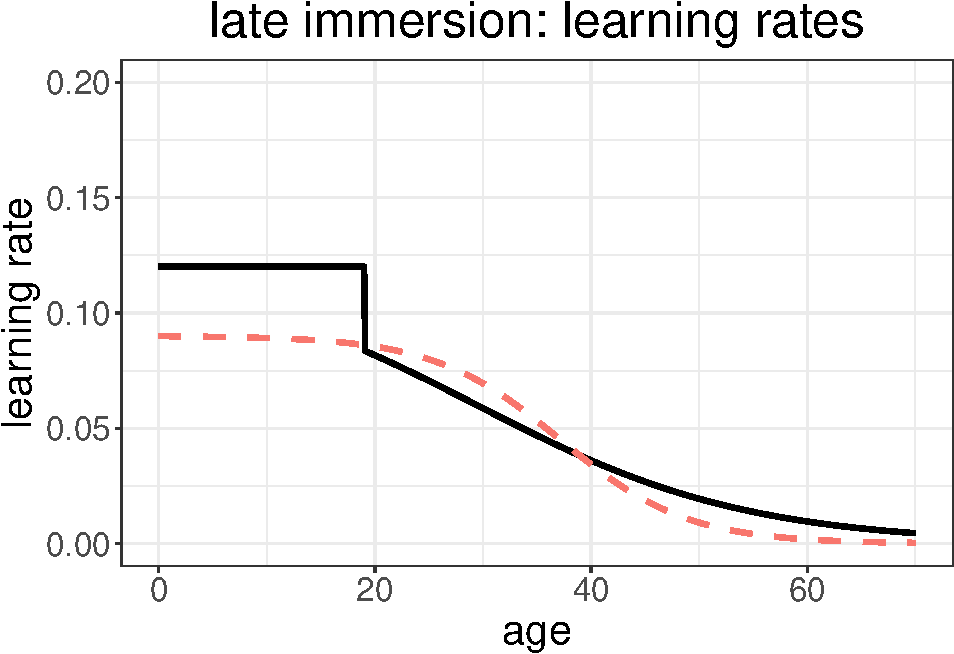
\includegraphics[width=0.48\linewidth]{SlikResponse_rmd_files/figure-latex/immersion-3} 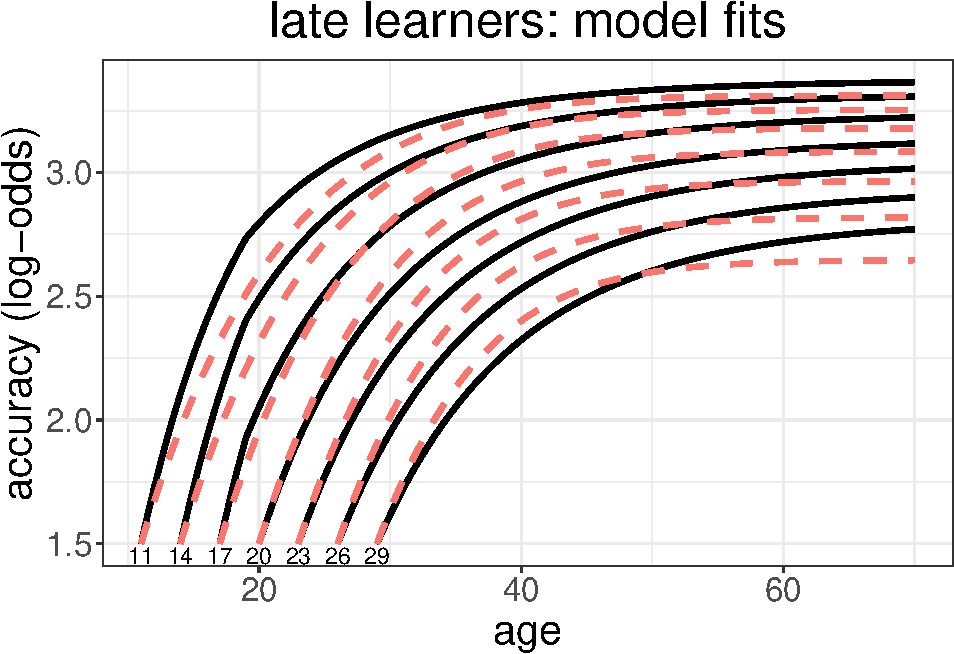
\includegraphics[width=0.48\linewidth]{SlikResponse_rmd_files/figure-latex/immersion-4} \caption{SSBH analyzed each learner group separately. Inferred age-related changes in learning curves (\emph{left panels}) and model fits (\emph{right panels}) for monolinguals only (\emph{top panels}) and simultaneous bilinguals only (\emph{bottom panels}). \emph{Solid black}: HTP's ELSD model. \emph{Dashed red}: SSBH's continuous model.}\label{fig:immersion}
\end{figure}

\hypertarget{comparing-age-related-declines}{%
\paragraph{Comparing Age-Related Declines}\label{comparing-age-related-declines}}

SSBH do note one other difference across learner groups: the age of onset of age-related decline is much later for monolinguals, simultaneous bilinguals, and early immersion learners than for the other two groups. They do not test whether this result is statistically significant, but it is. We can compare a model that fits each of the five learner groups separately with one that fits all simultaneously, finding that the former substantially outperforms the latter (\(AIC_diff\)=334; relative log-likelihood: 10\^{}72 to 1).

As already noted, to the extent that the models infer age-related decline for monolinguals, simultaneous bilinguals, or early immersion learners, these declines happen so late as to have minimal effect: all three groups are fit pretty well by exponential decay with a fixed learning rate. SSBH conclude that these three groups are not affected by age, whereas later immersion learners and non-immersion learners are affected by an age-related ``change in society and/or educational status'' (p.~18). (SSBH do not elaborate on why this change does not affect the other learner groups.)

These conclusions again depend on fallacies and statistical errors. First, while SSBH present these differences across learner groups as a novel observation, they were reported first by HTP. In particular, HTP in fact reported two sets of analyses showing that immersion learners who began before the age of 10 learn at least as rapidly and successfully as simultaneous bilinguals (HTP p.~270). Thus, SSBH merely present a third set of analyses indicating the same pattern. Since HTP also found that exponential decay provides a pretty good fit to native speaker learning curves, it follows that exponential decay also fits early immersion learners.

Second, HTP show the exact same thing for nonimmersion learners: learners who begin before around the age of 10 are indistinguishable, whereas later learners are slower and less successful. (SSBH do not report any analyses of their own.) Thus, the data actually strongly indicate that immersion and nonimmersion bilinguals are affected similarly by age -- exactly the opposite of what SSBH erroneously conclude.

Third and finally, SSBH are drawing very strong conclusions from small effects within a model that may not be sufficiently precise As already discussed, the ELSD model's method of instantiating asymmetric decline in learning rate can result in overly sharp declines, exemplified by the best ELSD fit to the full dataset (Fig. \ref{fig:HTP}). This will serve to distort model fits. Another distortion comes from the fact that the ELSD model requires the modeler to set maximum and minimum value for linguistic knowledge. Both HTP and SSBH used the range {[}1.5, 3.5{]} which is only approximately correct. However, as shown in Fig. \ref{fig:HTP}A\&B, the empirical range is a little wider than that. This limits how well the ELSD model can actually fit the data (cf.~Fig. \ref{fig:natives}, top right).\footnote{Frank (2018) has criticized the use of asymptotic models, given that many modern theories (especially construction grammars) posit that the set of grammatical structures is a) unbounded, and b) a moving target due to language change. While I agree in principle, so far in practice nobody has proposed a tractable non-asymptotic model. However, this does not absolve us from setting the asymptotes as precisely as possible.}

There are other imprecisions in the ELSD model, which I return to below. However, the two just mentioned are particularly significant and straightforward to address. Recently, Chen and Hartshorne (2021) introduced a more flexible model ``segmented sigmoid'' model that conjoins two sigmoids. This model can easily fit not only the curves fit by ELSD (and, by extension, SSBH's ``continuous'' model), but also smoother asymmetric curves of the types described in the last paragraph. In addition, I rescaled the model to cover the empirical range: {[}1.30, 3.70{]}.

I fit the resulting, more precise model to the extended dataset published by Chen and Hartshorne (2021). This dataset is substantially larger, with 319565 monolinguals, 41534 simultaenous bilinguals, 21174 immersion learners, and 543407 non-immersion learners. This larger dataset enables more precise measurement of the empirical learning curves, decreasing noise and improving precision of the model fits.

Fig. \ref{fig:seps} compares the results of fitting the revised model to all the data simultaneously and to each learner group individually. Above, I explained why I do not believe this is a particularly good test of SSBH's hypothesis, but it is the one they propose. Similarly, in order to evaluate SSBH's hypothesis on the grounds most favorable to it, I follow them in dividing the immersion group into ``early'' and ``late'' subgroups, but not the non-immersion group.

For four of the learner groups, fitting to the group individually does not much change the fit, with all models showing a sharp drop in the decay (``learning'') rate in late adolescence. The lone exception is monolinguals: fitting to only monolinguals does result in inferring a substantially later decline. While this result is significant (\(AIC_diff\) = 63), the impact on the model fit is again quite subtle. I return to this in the next and final section.



\begin{figure}
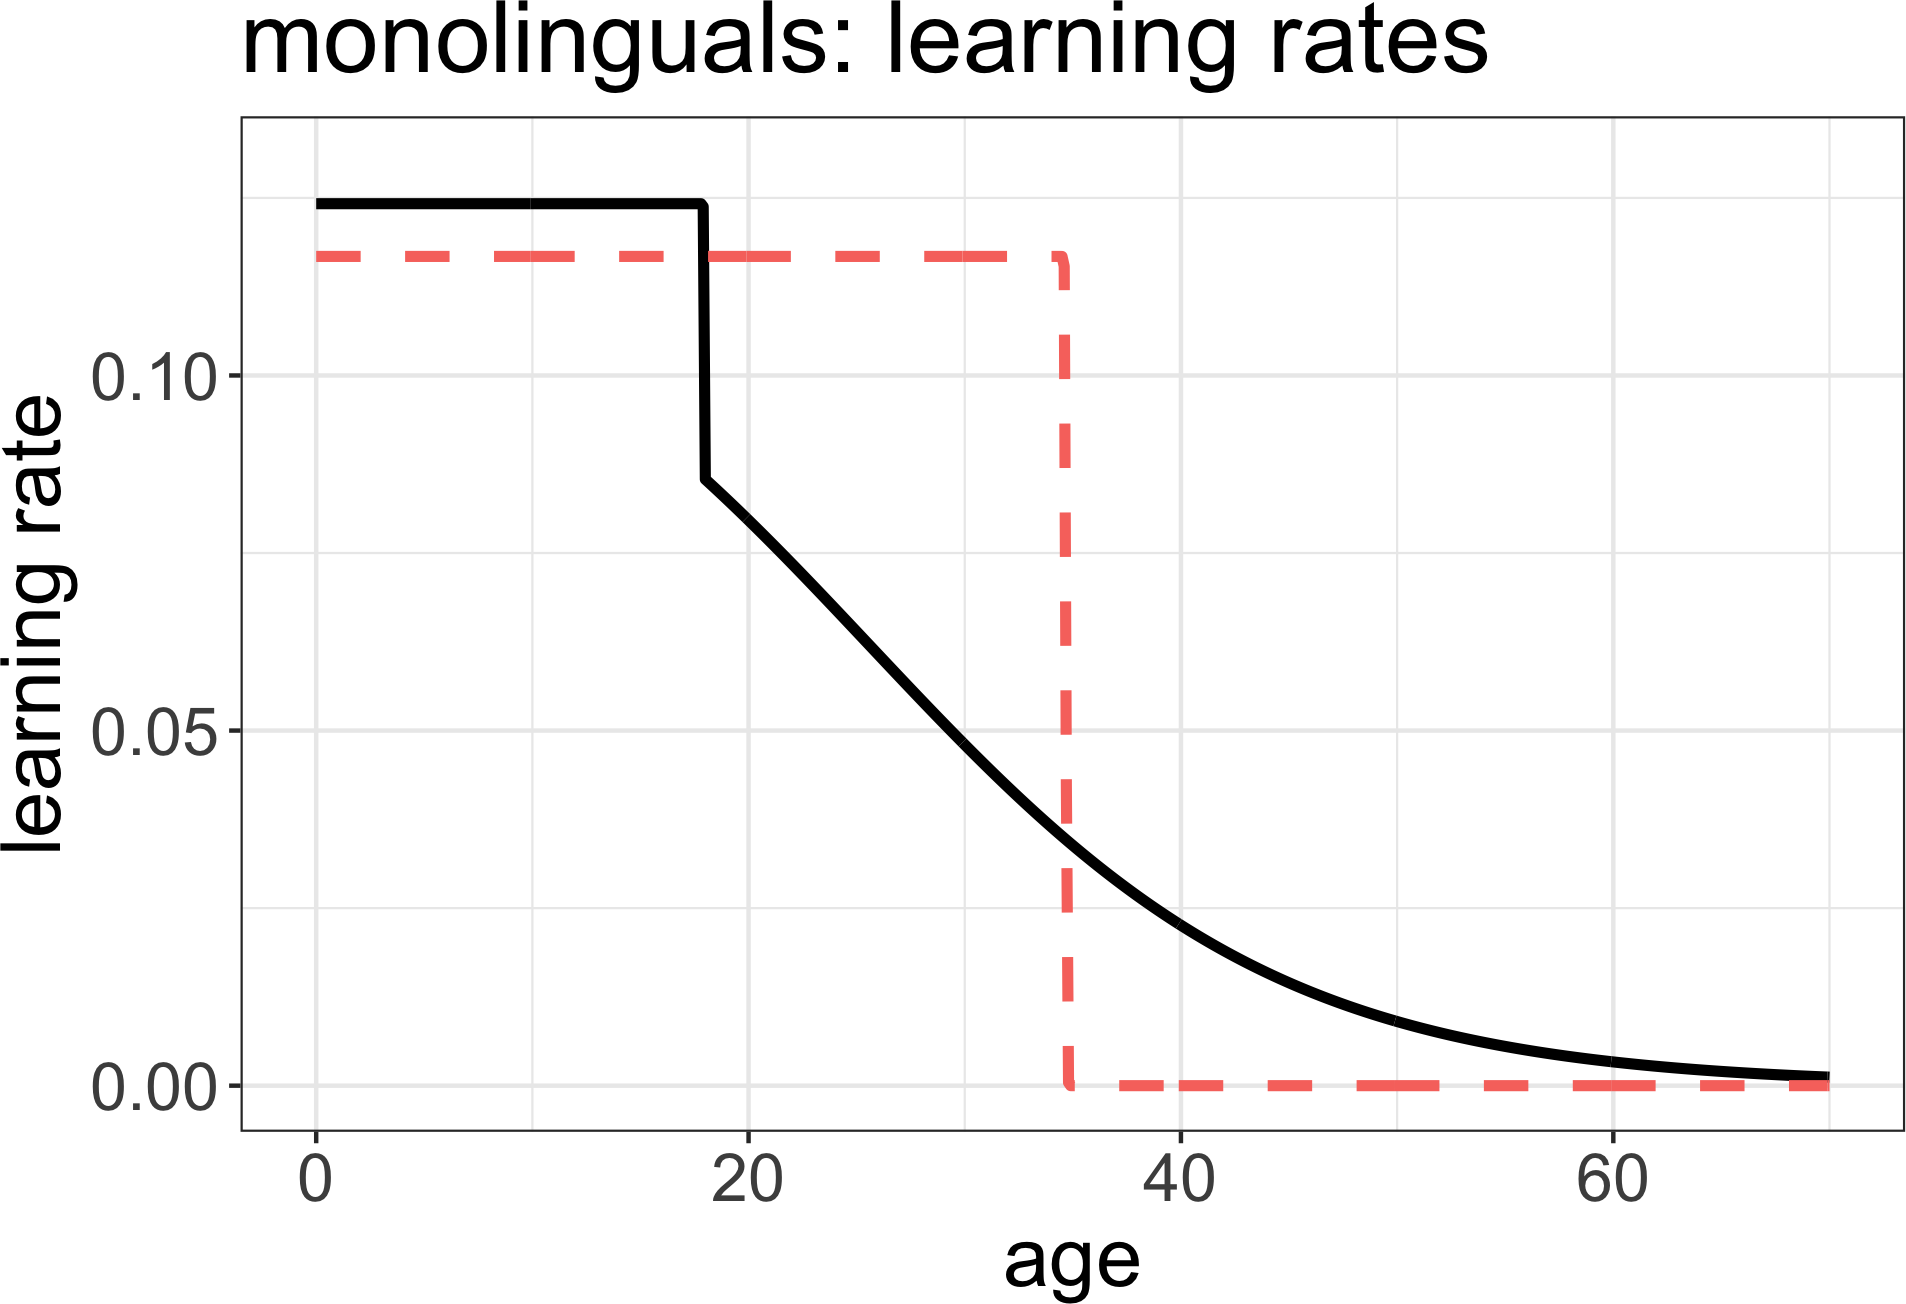
\includegraphics[width=0.4\linewidth]{SlikResponse_rmd_files/figure-latex/seps-1} 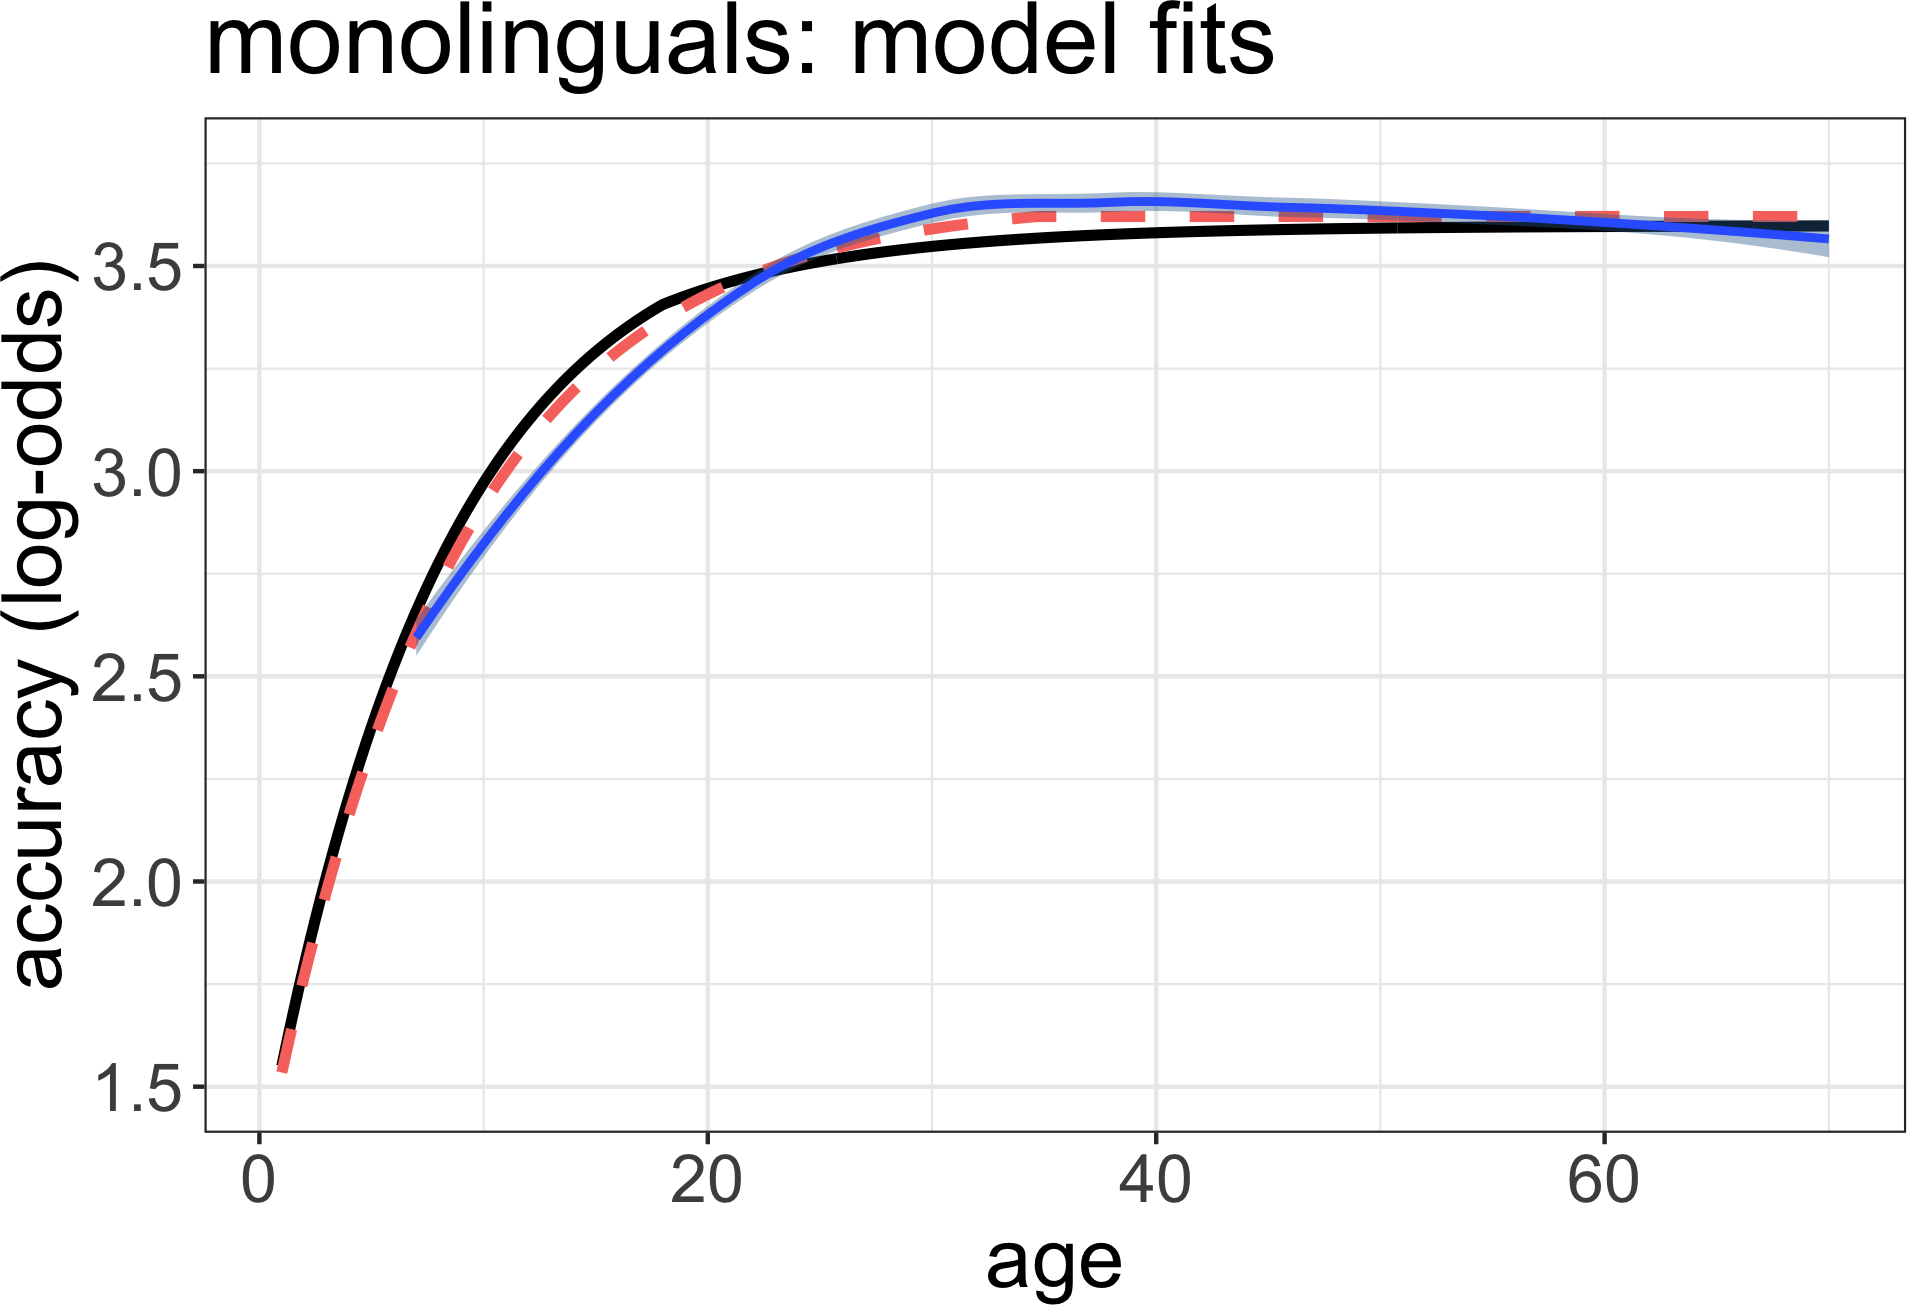
\includegraphics[width=0.4\linewidth]{SlikResponse_rmd_files/figure-latex/seps-2} 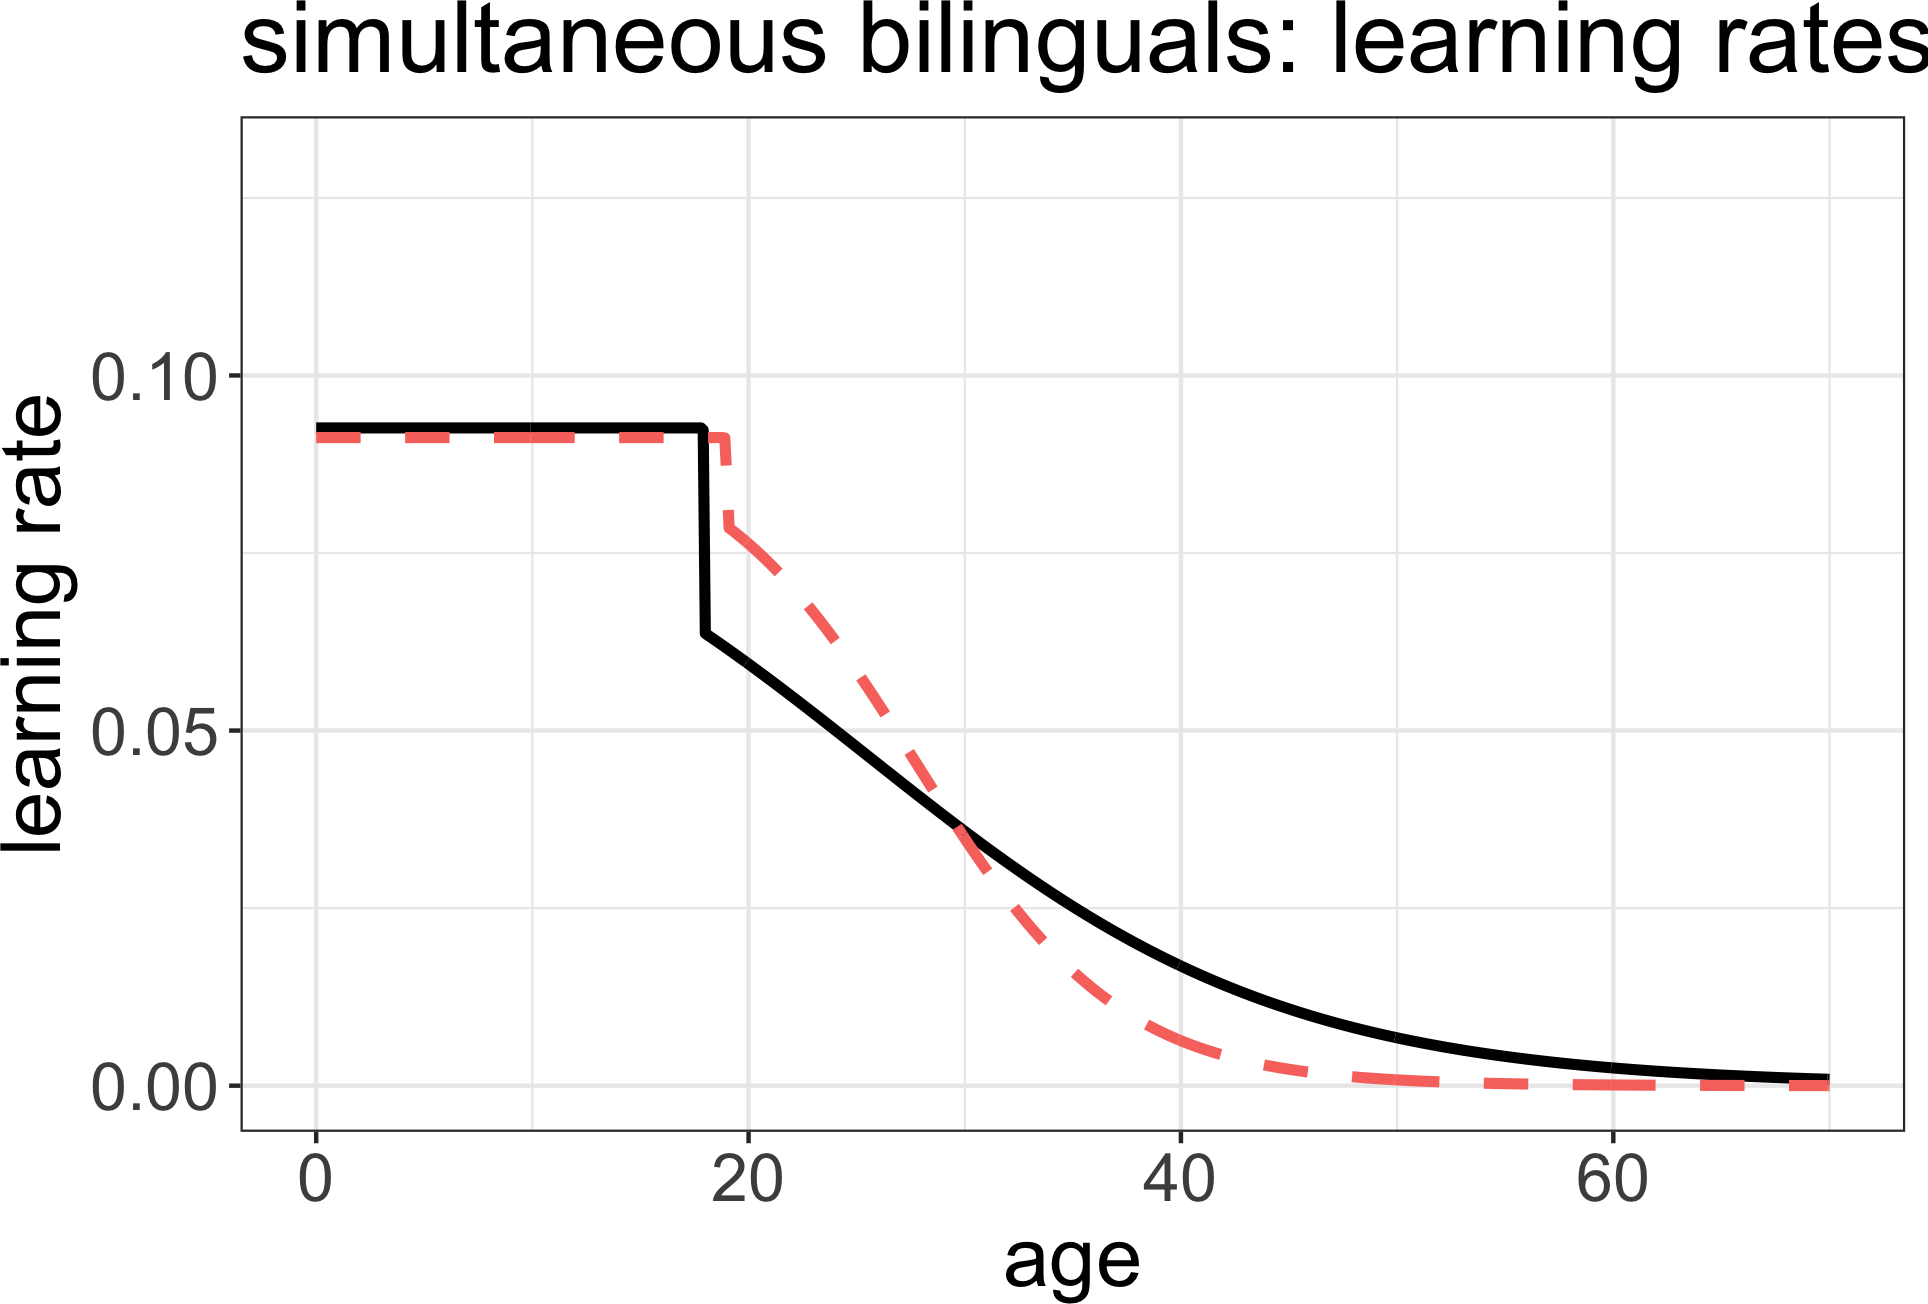
\includegraphics[width=0.4\linewidth]{SlikResponse_rmd_files/figure-latex/seps-3} 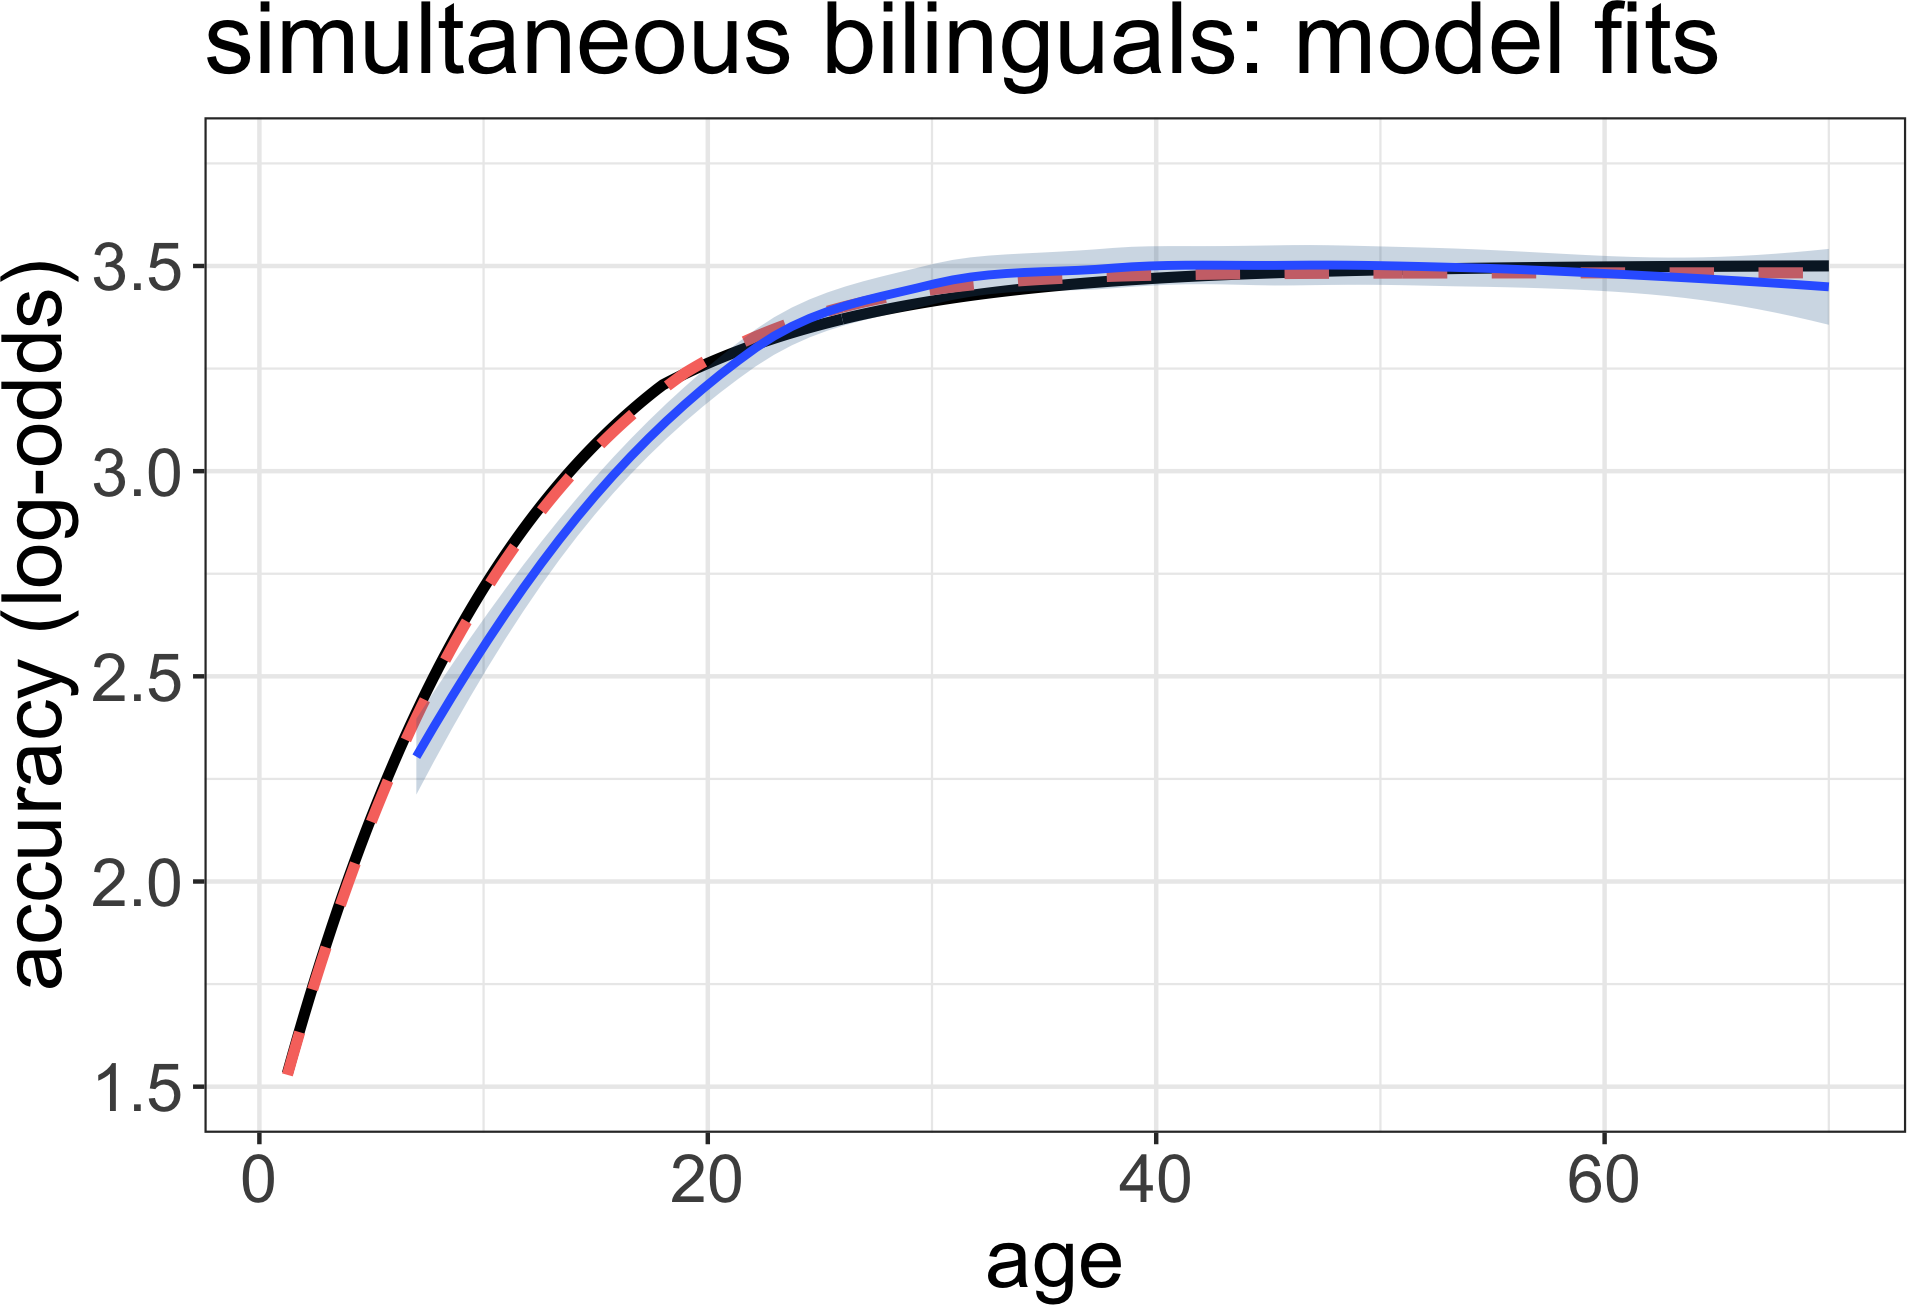
\includegraphics[width=0.4\linewidth]{SlikResponse_rmd_files/figure-latex/seps-4} 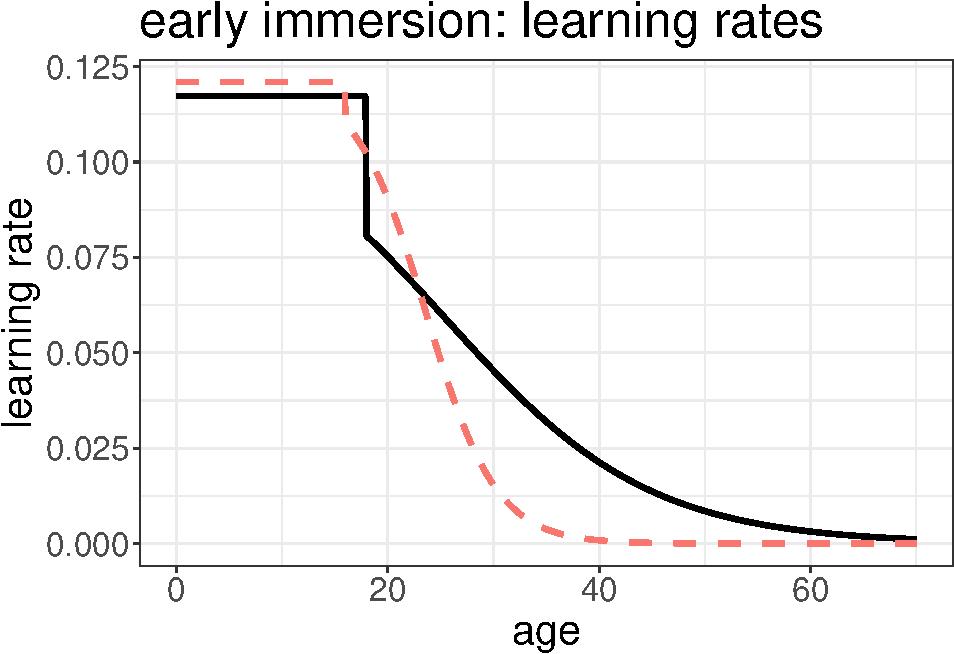
\includegraphics[width=0.4\linewidth]{SlikResponse_rmd_files/figure-latex/seps-5} 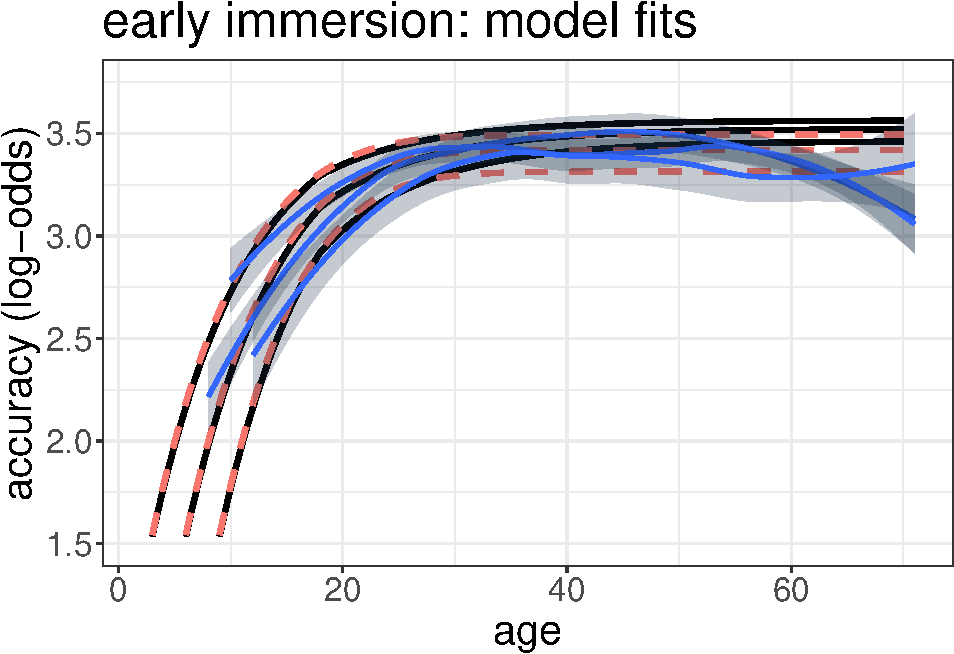
\includegraphics[width=0.4\linewidth]{SlikResponse_rmd_files/figure-latex/seps-6} 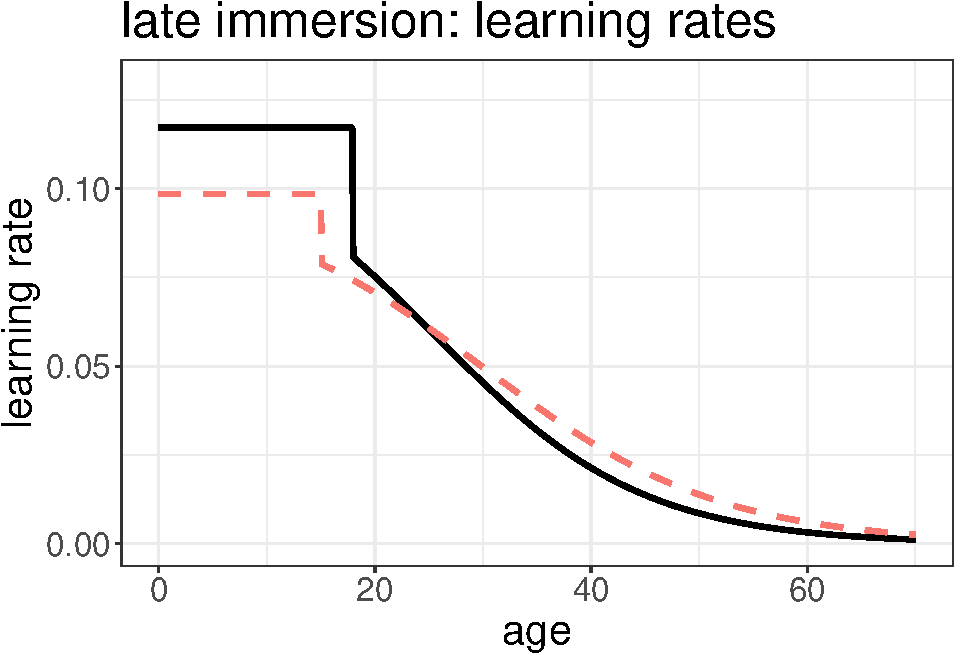
\includegraphics[width=0.4\linewidth]{SlikResponse_rmd_files/figure-latex/seps-7} 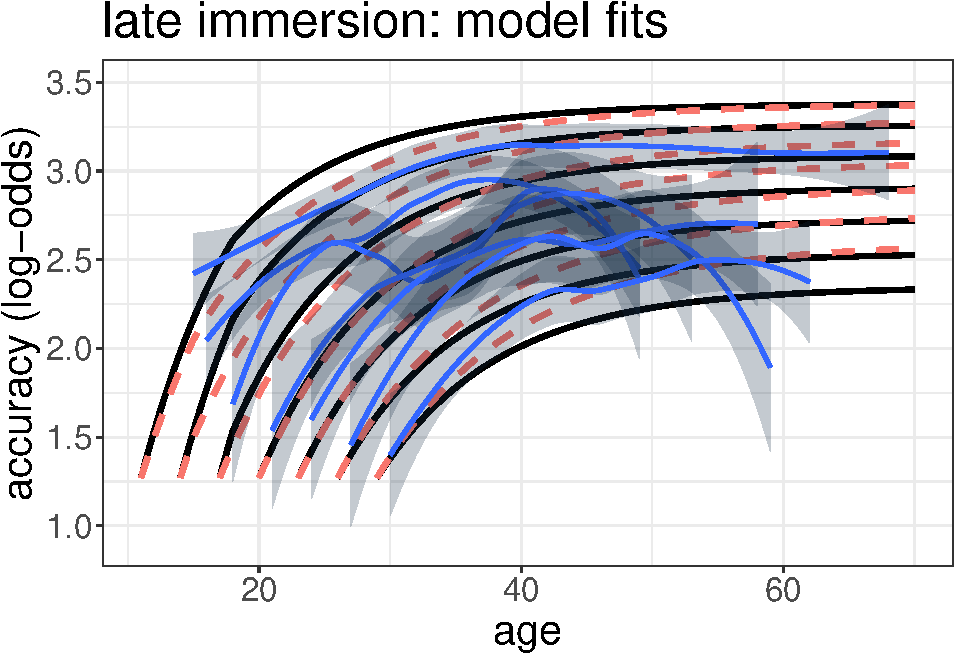
\includegraphics[width=0.4\linewidth]{SlikResponse_rmd_files/figure-latex/seps-8} 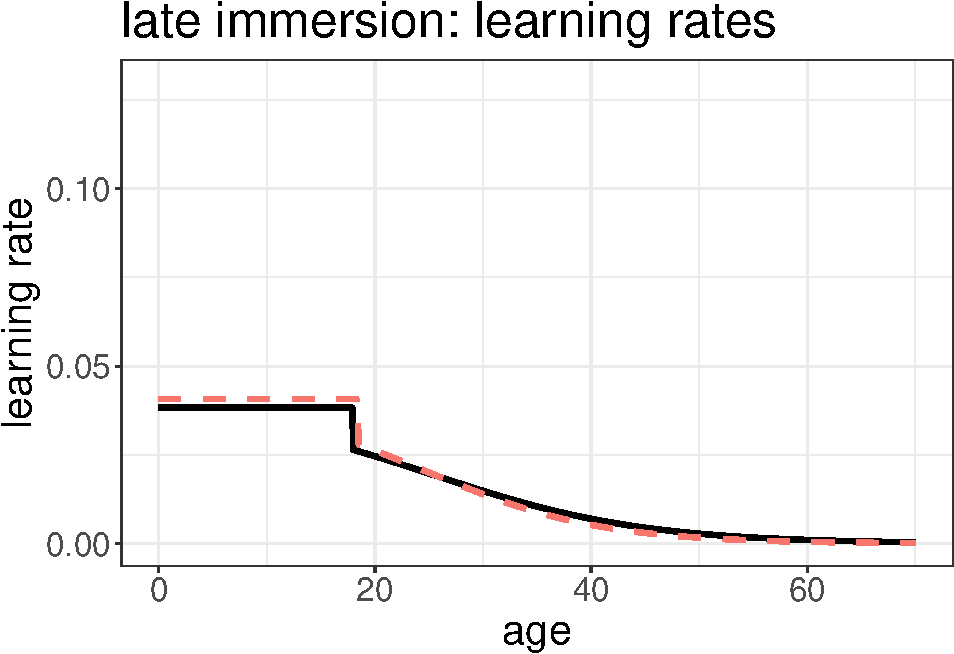
\includegraphics[width=0.4\linewidth]{SlikResponse_rmd_files/figure-latex/seps-9} 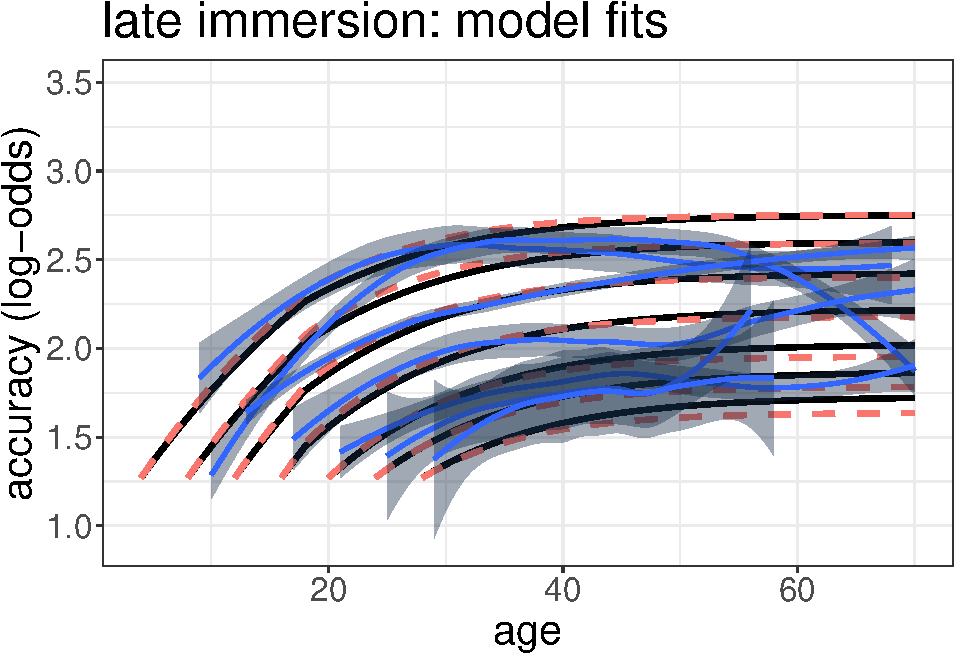
\includegraphics[width=0.4\linewidth]{SlikResponse_rmd_files/figure-latex/seps-10} \caption{Comparisons of the revised model trained on all data (solid black lines) and on individual learner groups (dashed red lines), and LOESS-smoothed data (blue lines with shaded 95\% confidence intervals). For nonimmersion learners, only a subset of curves are shown.}\label{fig:seps}
\end{figure}

\hypertarget{summary-and-conclusions}{%
\section{Summary and Conclusions}\label{summary-and-conclusions}}

SSBH suggest that HTP's data show that different learner groups show distinct effects of age on learning, with one group largely unaffected (monolinguals, simultaneous bilinguals, early immersion learners) and the other showing a marked decline in adolescence (late immersion learners, non-immersion learners). However, none of their arguments or results hold up under scrutiny. The paper contains dozens of factual misstatements and mathematical miscalculations. Their primary analysis (the comparison of the ``discontinuous'' and ``continuous'' models) does not actually test for a discontinuity, and the results are not significant.

After correcting their errors and improving the precision of their analyses, the results paint a very different picture from the one sketched by SSBH: when analyzed individually, all learner groups exhibit a sharp decline in learning ability in late adolescence, with the lone exception of monolinguals, who showed a somewhat later (but even more dramatic) decline. This difference has to be interpreted with caution: monolinguals are the fastest learners, and so they are least affected by the exact timing of age-related decline. Thus, with respect to SSBH's hypothesis, the best-case scenario is that all learner groups are equally affected by age, with the lone exception of monolinguals, who are, for reasons unknown, blessed. The worst-case scenario is that there are no differences at all.

Even the revised model does not fit the data perfectly. It has no previsions for senescence, which turns out to appear much earlier than had been visible in HTP's data (compare Fig. \ref{fig:HTP}A with Fig. \ref{fig:seps}, top): around age 35. Unfortunately, our original strategy of simply excluding older subjects will not work: excluding subjects older than 35 would vitiate our ability to study later learners. Similarly, the model cannot entertain age-related \emph{increases} in learning rate, even though these are clear in the present data and in prior work that this occurs in childhood (cf. Snow \& Hoefnagel-Höhle, 1978). The models assume learning is asymtotic, whereas Frank (2018) correctly notes that many modern theories (especially construction grammars) posit that the set of grammatical structures is a) unbounded, and b) a moving target due to language change.\footnote{I am sympathetic to this point. HTP only adopted asymptotic learning because a) we weren't able to develop anything else that was computationally tractable, and b) exponential decay fit the data pretty well.} The models assume that the differences in learning rate across learner groups (encapsulated by \(E\)) does not change with age, which is probably unrealistic -- especially if what \(E\) is capturing is differences in the quality \& quantity of the input.

Nonetheless, modulo two caveats I return to below, the model is not likely to be \emph{very} wrong. The model fits the data so well that any better-fitting model is likely to be a variation on the theme, not a radical departure. Indeed, many of the imprecisions described above are measurably small: for instance, grammatical knowledge declines between the ages of 35 and 70, but not by much. Indeed, two rounds of model improvement (here and in Chen and Hartshorne (2021)) have resulted in a clearer picture but not a substantially different picture.

The first caveat is that the model is limited by the data. While a lot of care went into creating HTP's quiz, I doubt that any 95-question quiz can assess an infinitely expressive human grammar precisely and without bias. If such a quiz can be created, we certainly lack the theoretical understanding of syntax needed to construct it at the moment. Moreover, HTP's probes meta-linguistic grammaticality judgments. This is certainly an important linguistic phenomenon -- the spectacular failure of late learners to acquire native-like meta-linguistic knowledge is part of what we wish to explain! -- but it certainly involves cognitive mechanisms not required for other linguistic phenomena, which themselves depend on cognitive mechanisms not needed for meta-linguistic judgment. To the extent this mechanisms are themselves affected by age, the picture will depend on which phenomenon we study.

The second caveat is that our modeling method estimates age-related change in learning rate. It does not assume -- nor can it test -- that this change is due to changes in a single mechanism. It could well reflect the aggregate effects of changes in multiple mechanisms that decline on different schedules.

All of which is to say that HTP and follow-up papers Slik et al. (2021) are just the start of a conversation. We will need many more studies of similar scale and scope to resolve all the open theoretical questions.

\clearpage

\hypertarget{references-cited}{%
\section*{References Cited}\label{references-cited}}
\addcontentsline{toc}{section}{References Cited}

\hypertarget{refs}{}
\begin{CSLReferences}{1}{0}
\leavevmode\vadjust pre{\hypertarget{ref-akaike1974new}{}}%
Akaike, H. (1974). A new look at the statistical model identification. \emph{IEEE Transactions on Automatic Control}, \emph{19}(6), 716--723.

\leavevmode\vadjust pre{\hypertarget{ref-birdsong2018plasticity}{}}%
Birdsong, D. (2018). Plasticity, variability and age in second language acquisition and bilingualism. \emph{Frontiers in Psychology}, \emph{9}, 81.

\leavevmode\vadjust pre{\hypertarget{ref-burnham1998practical}{}}%
Burnham, K. P., \& Anderson, D. R. (1998). Practical use of the information-theoretic approach. In \emph{Model selection and inference} (pp. 75--117). Springer.

\leavevmode\vadjust pre{\hypertarget{ref-chen2021more}{}}%
Chen, T., \& Hartshorne, J. K. (2021). More evidence from over 1.1 million subjects that the critical period for syntax closes in late adolescence. \emph{Cognition}, \emph{214}, 104706.

\leavevmode\vadjust pre{\hypertarget{ref-flege2019non}{}}%
Flege, J. E. (2019). A non-critical period for second-language learning. \emph{A Sound Approach to Language Matters: In Honor of Ocke-Schwen Bohn, Aarhus University. Open Access e-Book at Aurhus University Library}.

\leavevmode\vadjust pre{\hypertarget{ref-frank2018great}{}}%
Frank, M. C. (2018). With great data comes great (theoretical) opportunity. \emph{Trends in Cognitive Sciences}, \emph{22}(8), 669--671.

\leavevmode\vadjust pre{\hypertarget{ref-hartshorne2020massive}{}}%
Hartshorne, J. K. (2020). How massive online experiments (MOEs) can illuminate critical and sensitive periods in development. \emph{Current Opinion in Behavioral Sciences}, \emph{36}, 135--143.

\leavevmode\vadjust pre{\hypertarget{ref-Hartshorne2018}{}}%
Hartshorne, Joshua K. and Tenenbaum, Joshua B., \& Pinker, S. (2018). A critical period for second language acquisition: Evidence from 2/3 million English speakers. \emph{Cognition}, \emph{177}, 263--277. \url{https://doi.org/10.1016/j.cognition.2018.04.007}

\leavevmode\vadjust pre{\hypertarget{ref-Hernandez2021}{}}%
Hernandez, A. E., Bodet, J. P., Gehm, K., \& Shen, S. (2021). What does a critical period for second language acquisition mean?: Reflections on Hartshorne et al. (2018). \emph{Cognition}, \emph{206}, 104478. \url{https://doi.org/10.1016/j.cognition.2020.104478}

\leavevmode\vadjust pre{\hypertarget{ref-van2021critical}{}}%
Slik, F. van der, Schepens, J., Bongaerts, T., \& Hout, R. van. (2021). Critical period claim revisited: Reanalysis of hartshorne, tenenbaum, and pinker (2018) suggests steady decline and learner-type differences. \emph{Language Learning}.

\leavevmode\vadjust pre{\hypertarget{ref-snow1978critical}{}}%
Snow, C. E., \& Hoefnagel-Höhle, M. (1978). The critical period for language acquisition: Evidence from second language learning. \emph{Child Development}, 1114--1128.

\leavevmode\vadjust pre{\hypertarget{ref-vanhove2013critical}{}}%
Vanhove, J. (2013). The critical period hypothesis in second language acquisition: A statistical critique and a reanalysis. \emph{PloS One}, \emph{8}(7), e69172.

\leavevmode\vadjust pre{\hypertarget{ref-wagenmakers2007practical}{}}%
Wagenmakers, E.-J. (2007). A practical solution to the pervasive problems of p values. \emph{Psychonomic Bulletin \& Review}, \emph{14}(5), 779--804.

\end{CSLReferences}


\clearpage



\begin{appendix}
\section{}
SSBH make a number of factual misstatements and mathematical errors.

In Table 2 and surrounding text, they report some discrepancies betweern
the number of subjects per condition for the critical analyses reported
by HTP (p.~266) and in SSBH's own analyses. The problem seems to be that
they ran their exclusions in a different order from HTP, despite basing
their analyses on HTP's code. Specifically, both papers bin subjects by
age, age of acquisition, and condition. We then restrict analyses to
consecutive ages for which there were at least 10 parrticipants in a
5-year window. HTP excludes subjects over the age of 70 before this
binning, whereas SSBH exclude subjects over the age of 70 \emph{after}
binning. This means subjects over teh age of 70 count towards binning
for SSBH but not for HTP, allowing inclusion of more bins for SSBH.
Thus, as they report, they end up with 38 more total included subjects.

SSBH report that HTP defined immersion learners as either simultaneous
bilinguals or ``later learners who spent at least 90\% of their life in
an English-speaking country'' (SSBH, p.~7). In fact, later immersion
learners were required to have spent at least 90\% of their life
\emph{since starting to learn English} in an English speaking country
(HTP, p.~266). This error is a bit of a head-scratcher: analyses include
immersion learners who began learning English as late as 30, which would
require them to be at least 300 years old at time of testing. Similarly,
they mistakenly report that non-immersion learners were those ``who
spent at most 10\% of their life in an English-speaking country'' (SSBH,
p.~8), whereas the actual definition is ``spent at most 10\% of
post-exposure life in an English-speaking country and no more than 1
year in total'' (HTP, p.~266).

Probably because of their confusion about how subject groups were
defined, SSBH mistakenly report that ``more than 100,000 language
learners in the HTP database could not be classified as belonging to one
of the four groups \emph{because key information was missing}''
(emphasis added; p.~20). They assert that this high rate of missing data
should cast doubt on the validity/accuracy of the HTP data. However,
these subjects were not excluded for missing data but rather for having
amounts of immersion intermediate between the ``immersion'' and
``non-immersion'' learners (see sentence spanning pp.~266-267).

SSBH misdescribe the stimuli. They report that HTP's test included 132
items, of which 95 were used for analysis ``based on the criterion that
at least 70\% of the native English-speaking adults gave the same
response'' (SSBH, p.~8). In fact, the criterion was that the same
response was given by at least 70\% of native English-speaking adults in
each of 13 dialect groups (HTP, p.~267). The reason was to exclude items
for which there was significant dialectal variation. They also assert
that HTP measures accuracy on the grammaticality judgment test on a
scale of 0 to 1, reflecting ``a proportion of correct answers (g)''
(SSBH, p.~7). In fact, \emph{g} represents log-odds accuracy on HTP's
syntax test and runs from 1.5 to 3.5 (see HTP Supplementary Materials,
p.~2). They misstate how HTP (and, it appears, they) calculated
log-odds, asserting that it was based on proportion
(\emph{log(p/{[}1-p{]})}) (SSBH, p.~7) rather than the empirical logit
transformation (\emph{log((ncorrect+.5)/(nincorrect+.5))}).

SSBH use Akaike Information Criterion (AIC) for model comparison, but in
almost every case appear to have miscounted the number of parameters in
the models (a key part of calculating AIC). For most of their analyses,
the ``continuous'' model has 4 free parameters (\(r_0\), \(\alpha\),
\(\delta\), and the error variance), though in all but one case, they
count it as having 5. The ``discontinuous'' model has one additional
free parameter (\(t_c\)) but for some reason is counted as having 7. The
exceptions are as follows: In the case of the monolingual analysis, they
correctly assign the continuous model 4 parameters, but again over-count
the discontinuous model (6 instead of 5). When fit to all data, there
are 3 additional parameters (the three E parameters), which should give
the ``continuous'' model 7 parameters (which they code correctly) and
give the ``discontinuous'' model 8 (they count 9).

(Note that they explain in Footnote 5 that ``the discontinuous model
needs to fit three components, the continuous model only one (cf.~Figure
1). That explains the difference of two degrees of freedom.'' It is not
possible to count degrees of freedom by inspecting a graph, and the
numbers here do not match the numbers in their code.)

These errors tend to overstate the evidence for the ``continuous''
model. For instance, the relative likelihood for the monolingual
analyses in their Table 3 is reported as 0.16. Using the correct number
of parameters, it is 0.30. That is, using AIC correctly, rather than the
``continuous'' model being nearly 7 times more likely, it is only about
3 times more likely. (Strangely, using SSBH's counting of parameters,
the ratio is actually 0.08; I have not yet identified the source of that
error.)

When replicating one of HTP's analyses, they report that they obtained
``a slightly higher \(R^2\) value of .92 (HTP found .89)'' (SSBH,
p.~10). This likely reflects the fact that while HTP report
cross-validated \(R^2\) values in order to address over-fitting, SSBH do
not. This will necessarily result in higher \(R^2\) values. It is not
clear whether this was an oversight or a misunderstanding of how
curve-fitting works. In a personal communication, van der Slik suggested
that because they ran the optimization algorithm for more iterations
than did HTP, this should obviate the need for cross-validation. This is
exactly backwards. It is a necessary fact that the more closely the
model is fit to the data, the worse over-fitting gets. In any case, the
result is that the \(R^2\) values must be treated with caution: a
particular model may achieve a better \(R_2\) simply due to overfitting.

In Footnote 7, they write that Chen and Hartshorne ``did not test if the
application of their segmented model has resulted in a significant
improvement in model fit as compared to the continuous model or even the
original HTP discontinuous model.'' In fact, we provided two such
metrics. First, the model fits available to ELSD are a proper subset of
those available to Chen \& Hartshorne's segmented sigmoid model, and
thus fitting the revised model is \emph{per se} a comparison of model
fit. Second, Chen and Hartshorne also provide cross-validated R\^{}2
statistics for both models, which corrects for model complexity.

Note that this list is probably not complete. In particular, I did not
check all (or even most) of their calculations. I focused on those
critical the present discussion or which contained easy-to-spot
mistakes.
\end{appendix}

\end{document}
